 \RequirePackage[l2tabu,orthodox]{nag} % for package advice

% TODO: decide if one-sided/two-sided
%\documentclass[headsepline,footsepline,footinclude=false,fontsize=11pt,paper=a4,listof=totoc,bibliography=totoc,BCOR=12mm,DIV=12]{scrbook} % two-sided
\documentclass[headsepline,footsepline,footinclude=false,oneside,fontsize=11pt,paper=a4,listof=totoc,bibliography=totoc]{scrbook} % one-sided

\PassOptionsToPackage{table,svgnames,dvipsnames}{xcolor}

% general/language
\usepackage[utf8]{inputenc}
\usepackage[T1]{fontenc}
\usepackage[sc]{mathpazo}
\usepackage[american]{babel}
\usepackage[autostyle]{csquotes}
\usepackage[%
  backend=bibtex,
  url=false,
  doi=false,
  style=numeric,
  giveninits,
  sorting=none,
  maxnames=2
]{biblatex}
\usepackage{booktabs} % for rulers in tables
\usepackage[final]{microtype} % for \microtypesetup{protrusion=true}
\usepackage[hidelinks, breaklinks = true]{hyperref} % hidelinks removes colored boxes around references and links, breaklinks allows linebreak in e.g. list of figures for long captions
%\usepackage[toc,nonumberlist,acronym]{glossaries} % TODO: remove if glossary not needed

% math
\usepackage{amsmath}
\usepackage{algorithm} %for algorithm environment
\usepackage{algpseudocode} %for algorithm environment
\usepackage{units} % for units
%\usepackage{scrhack} % necessary for listings package
%\usepackage{listings}
\usepackage[nameinlink]{cleveref}

% graphics
\usepackage{graphicx}
\usepackage{psfrag}
\usepackage{subfig}
%\usepackage{epstopdf}
%\usepackage{tikz}
%\usepackage{pgfplots}
%\usepackage{pgfplotstable}





% Basic information for cover & title page
\newcommand*{\getUniversity}{Technical University of Munich} %{Technische Universität München}
\newcommand*{\getFaculty}{Department of Informatics}
\newcommand*{\getTitle}{Microcontroller based Object Tracking for Room Monitoring}
\newcommand*{\getTitleGer}{Objekt Tracking auf einem Mikrocontroller zur Raumüberwachung}
\newcommand*{\getAuthor}{Chenyuan Zhao}
\newcommand*{\getDoctype}{Master's Thesis in Informatics}
\newcommand*{\getSupervisor}{Prof. Dr. Michael Gerndt}
\newcommand*{\getAdvisor}{Prof. Dr. Michael Gerndt}
\newcommand*{\getSubmissionDate}{15.10.2021}
\newcommand*{\getSubmissionLocation}{Munich}

\newcommand{\arstretch}[1]{\renewcommand{\arraystretch}{#1}} %to change the row spacing in tables
% TODO: add custom commands etc.

% Settings for bibliography
\bibliography{content/ref,content/overviewref,content/cvref,content/links}

% Settings for fonts
\setkomafont{disposition}{\normalfont\bfseries} % use serif font for headings
\linespread{1.05} % adjust line spread for mathpazo font

% Settings for glossaries
%\renewcommand{\glsnamefont}[1]{\normalfont\bfseries #1} % use serif font for glossary entry titles
%\makeglossaries{}

% Settings for pgfplots
%\pgfplotsset{compat=1.9} % TODO: adjust to your installed version
%\pgfplotsset{
%  % For available color names, see http://www.latextemplates.com/svgnames-colors
%  cycle list={CornflowerBlue\\Dandelion\\ForestGreen\\BrickRed\\},
%}

% Settings for lstlistings
%\lstset{%
%  basicstyle=\ttfamily,
%  columns=fullflexible,
%  autogobble,
%  keywordstyle=\bfseries\color{MediumBlue},
%  stringstyle=\color{DarkGreen}
%} 
% \newglossaryentry{computer}
{
  name=computer,
  description={is a machine that\ldots}
}
 % TODO: uncomment if glossary needed
% \newacronym{tum}{TUM}{Technische Universität München}
 % TODO: uncomment if list of abbreviations needed
\begin{document}
\begin{titlepage}
  % HACK for two-sided documents: ignore binding correction for cover page.
  % Adapted from Markus Kohm's KOMA-Script titlepage=firstiscover handling.
  % See http://mirrors.ctan.org/macros/latex/contrib/koma-script/scrkernel-title.dtx,
  % \maketitle macro.
  \oddsidemargin=\evensidemargin\relax
  \textwidth=\dimexpr\paperwidth-2\evensidemargin-2in\relax
  \hsize=\textwidth\relax

  \centering

  \vspace{40mm}
  
\includegraphics[width=40mm]{./figures/tum}

  \vspace{5mm}
  {\LARGE \MakeUppercase{\getUniversity{}}}\\

  \vspace{5mm}
  {\Large \MakeUppercase{\getFaculty{}}}\\

  \vspace{20mm}
  {\Large \getDoctype{}}

  \vspace{15mm}
  {\huge\bfseries \getTitle{}}

  \vspace{15mm}
  {\LARGE \getAuthor{}}

  \vspace{20mm}
  %
\includegraphics[width=20mm]{logos/faculty}
	
\end{titlepage}


\frontmatter{}
\begin{titlepage}
  \centering

  \vspace{40mm}
  
\includegraphics[width=40mm]{./figures/tum}

  \vspace{5mm}
  {\LARGE \MakeUppercase{\getUniversity{}}}\\

  \vspace{5mm}
  {\Large \MakeUppercase{\getFaculty{}}}\\

  \vspace{20mm}
  {\Large \getDoctype{}}

  \vspace{15mm}
  {\huge\bfseries \getTitle{}}

  \vspace{10mm}
  {\huge\bfseries \getTitleGer{}}

  \vspace{15mm}
  \begin{tabular}{l l}
    Author: & \getAuthor{} \\
    Supervisor: & \getSupervisor{} \\
    Advisor: & \getAdvisor{} \\
    Submission Date: & \getSubmissionDate{} \\
  \end{tabular}

  \vspace{20mm}
  %
\includegraphics[width=20mm]{logos/faculty}
\end{titlepage}

\thispagestyle{empty}
\vspace*{0.65\textheight}
\noindent
I confirm that this master's thesis is my own work and I have documented all sources and material used. \\\\
Ich versichere, dass ich diese Master's Thesis selbständig verfasst und nur die angegebenen Quellen und Hilfsmittel verwendet habe.

\vspace{15mm}
\noindent
\getSubmissionLocation{}, \getSubmissionDate{} \hspace{5cm} \getAuthor{}

\cleardoublepage{}

\addcontentsline{toc}{chapter}{Acknowledgments}
\thispagestyle{empty}

\vspace*{2cm}

\begin{center}
{\usekomafont{section} Acknowledgments}
\end{center}

\vspace{1cm}

I want to give a big thank to my supervisor Prof. Michael Gerndt. He gave me the initial idea of this thesis. During the project phase he also followed my progress continuously and gave instant feedback. I found the discussions between us are quite happy and enjoyable. Every time we talked, I felt my goal becomes more concrete.

I would like to thank the Espressif community as well. Espressif is the manufacturer of the microcontroller I used in my thesis but they are definitely more than that. Thanks to the help of the community I have met many nice people who gave me hints to solve the issues occurred in the implementation. Their vivid working atmosphere and confidence in their own products are another two reason that I decided to join in. If thing works smoothly I will start the job at Espressif from this December.

And also thanks to my roommates. The Corona pandemic is an unforgettable expedience in my lifetime and it has bounded us closer. After three years of living together we are finally going to tear apart. I will miss you!

And finally thanks for my parents. They have financed my study abroad in Germany. I miss them so much and I will go home soon! 

\cleardoublepage{}

\chapter{\abstractname}
Counting human targets in buildings and rooms has many applications, such as elder care, heating optimization, and security. To protect the privacy of monitored humans, a low-resolution IR camera is placed at the top of the doorway to count enter and exit events. The collected images are interpolated and human objects are segmented from the background according to their temperature difference. The separated human targets are represented as binary blobs and further abstracted to centroids and central points. The human targets are associated with their respective trajectories by the nearest neighbor method and a filter. The results show an average of 95\% accuracy in the test environment and 81\% accuracy in the real environment. The algorithm is deployed on an inexpensive ESP32 microcontroller to reduce the cost. 
\microtypesetup{protrusion=false}
\tableofcontents{}
\microtypesetup{protrusion=true}

\mainmatter{}
\input{content/introduction}
\chapter{Literature Review} \label{ch:review}
Low-resolution thermopile-array sensors (LR-TAS) have been widely used in health-caring and indoor monitoring because of the feature of preserving privacy. According to the final objective, the related literature could be roughly classified into three categories: indoor localization and gesture estimation \cite{multi,karayaneva2018use,jeong2014probabilistic},
room surveillance \cite{gonzalez2013using,thermosense,basu2015tracking,IRTAS16x4}
or human object tracking and event counting \cite{mika,firstflow,melexis,virtualtrack}.
Most of the literature proposed a two-layers algorithm structure, which consists of an object detection layer and an activity classification layer. Regardless of the different final goal of the researches, several similar ideas are found in the object detection algorithms, which has inspired our design. The later data processing procedure is more task-specific and only the literature in the last category is highly related to our design.

Before we dive into the related literature, it is worth mentioning that there are already several commercial products that could track and count humans \cite{irisys,flir}. But the work principles of these products are not revealed. Moreover, they cannot output an articulate number of human counts and are often applied in mass population monitor for example in supermarkets.

\section{Detection Algorithms}
In the active pixel detection phase, the algorithm needs to distinguish a human from the background, namely to answer the question of ``Which pixels are occupied by a human?''

\citeauthor{mashiyama2015activity} \cite{mashiyama2015activity} rearrange the pixels by their reading values in descending order, and take a heuristic that the first $n$ pixels could be human, having a prior knowledge that a human usually takes up $n$ pixels in a scene. They also compare the average temperature of the first $n$ pixels with the rest pixels, only when the difference is large enough the first $n$ pixels are considered a human. This method has several drawbacks. The most obvious issue is that it can only detect one person. Moreover, the algorithm depends heavily on the prior knowledge threshold $n$, so it lacks the flexibility to detect different people with different figures. Finally, \citeauthor{trofimova2017indoor} \cite{trofimova2017indoor} has re-conducted the research and pointed out that it is very hard to determine the threshold.

\citeauthor{trofimova2017indoor} \cite{trofimova2017indoor} has also proposed their detection algorithm, which makes use of the on-board thermistor to estimate the environment temperature. They found that there is an approximately linear relation between the IR array temperature and the thermistor temperature, which indicates that any higher reading that breaks this linear relation is probably caused by a human. Since the sensor they use has a reading deviation up to $\pm 2.5^{\circ}C$, a larger deviation from the thermistor temperature is considered a activated pixel. This method is able to detect activated pixels individually. But from temperature readings alone, an IR-TAS cannot distinguish humans from other heat emitters such as computers or heaters.

Another way to separate a human from the background is to fully exploit the whole image frame. If a human is the only heat source in a thermal image, it is almost safe to assume that the body temperature is higher than the ambient temperature. Therefore, the human body and the background are naturally separated by temperature. Otsu's method could be applied to each frame individually to find out a threshold, such that pixels with a higher temperature are considered occupied by a human \cite{firstflow}.

Otsu's method provides good segmentation result but its low speed may be a drawback when real-time performance is required. The average temperature and standard deviation of a thermal image could also be used to calculate the threshold between fore- and backgrounds. \citeauthor{virtualtrack} \cite{virtualtrack} have proposed a simple algorithm based on the average temperature: any pixels with a temperature in the range of average temperature $\pm 3.0^\circ C$ are regarded as potential human objects and the rest pixels in the same frame are regarded as background.
%TODO: 解释一下virtual track作者如此选定阈值的原因
They further calculate the average temperature of fore- and background respectively, denoted as $T_o$ (object temperature) and $T_a$ (ambient). Next, a measurement temperature ($T_m$) is calculated by the following formula \autoref{eq:segmentbyavg}, where $S_o$ is the size of the object and $S_p$ is the total pixel number of one frame. A pixel that is $3^\circ C$ higher than $T_m$ is regarded as non-human heat source and will be excluded from object list.
\begin{equation}\label{eq:segmentbyavg}
  T_m = T_a + (T_o-T_a)*\frac{S_o}{S_p}
\end{equation}

Similarly, \citeauthor{jeong2014probabilistic} \cite{jeong2014probabilistic} purpose a global adaptive threshold using information of a single image frame. They exploit the fact that a too low standard deviation of an thermal image suggests it contains noises only. The purposed threshold is shown in \autoref{eq:segmentbystd}, where Max and Mean are the maximum and mean value in one frame, and SD is the standard deviation.
\begin{equation}\label{eq:segmentbystd}
  Threshold = (Max-Mean)*\left(0.025+\frac{0.85}{Max-Mean+1}\right) + Mean - 0.7\times SD
\end{equation}

Beside the aforementioned methods, a large group of detection algorithms fall into background substraction \cite{backgroundsubsurvey}, see \autoref{fig:backgroundsub}. This method maintains a background model in the processor's memory. A pixel is regarded active if its reading deviates from the stored background significantly. Instead of a global threshold, background substraction allows different regions of a camera FOV having different thresholds, which may be useful when there is a known heat source that should be ignored. Though the background substraction technique is more commonly used in RGB image data, transferring it to thermal image data also shows impressive results.
\begin{figure}
  \centering
  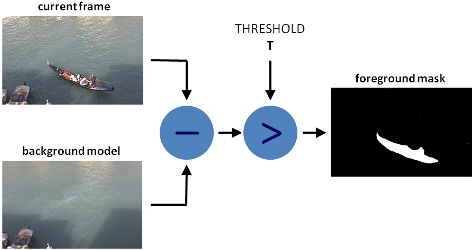
\includegraphics[width=0.8\textwidth]{figures/Background_Subtraction.png}
  \caption{A general idea of background substraction. Credit: \cite{opencvBackgroundSub}}\label{fig:backgroundsub}
\end{figure}

A simple implementation of background substraction is comparing the input image with a fix background. \citeauthor{basu2015tracking} \cite{basu2015tracking} collect more than 100 sample frames without humans, and use the average temperature as the background reference. \citeauthor{firstflow} \cite{firstflow} measure the background temperature only once when the device starts up, and take the assumption that the thermal background remains stable in a long term afterwards.

A fixed background may give acceptable result when the ambient temperature in the test environment does not vary. Under most circumstances, a background model that could adapt to the varying environment is desired. This could be done by a continuous update of the background pixels. After the fore- and background segmentation of each image frame, those pixels that do not exceed the background temperature will be merged into the background \cite{melexis,IRTAS16x4}, while those pixels that are considered as object do not contribute to the background model. The related formula is shown in \autoref{eq:backgroundupdate}:
\begin{equation} \label{eq:backgroundupdate}
\begin{split}
\mu_n[\mathbf{x}] & = \mathbf{1}\left(T_n[\mathbf{x}]\in B\right)\left[\alpha T_n[\mathbf{x}]+(1-\alpha)\mu_{n-1}[\mathbf{x}]\right]
  \\&+\mathbf{1}\left(T_n[\mathbf{x}]\in F\right) \mu_n[\mathbf{x}]
\end{split}
\end{equation}
where fore- and background are denoted as $F$ and $B$ respectively, $\mathbf{1}(\cdot)$ is the indicator function, and $\alpha \in (0,1)$ is the update rate.

The dynamic background learning method will dissolve an object that does not move for a long time into the background, which may be an advantage and drawback at the same time. When there is an unexpected non-human heat source in the camera view, the unanimated object could be ignored and do not influence detection judgements. On the other hand, a human will also be undesirably ignored if he stays still, which may brings about difficulties to the following algorithms. In order to detect humans only, \citeauthor{thermosense} \cite{thermosense} attached a PIR (passive infrared) sensor to their project in addition to the IR camera. PIR sensors are based on a principle of pyroelectric that is different from thermopile and can only detect heat movements. The authors assume that humans will not keep still for 15 minutes. The thermal camera will only capture and update the background if the PIR sensor does not sense a movement in such a period.

Finally, some researchers have explored machine learning (ML) methods for human object detection \cite{multi,karayaneva2018use}. But these methods will not be elaborated in this section because we want to concentrate on traditional CV methods.

\section{Tracking Algorithms}
After the human objects are detected and located, the task of a tracking algorithm is to assign a consistent label to the same object throughout the sequence of video images \cite{tang2010hybrid}. Following a bottom-up approach, four questions need to be answered to define an object tracker: what's the suitable (shape) representation of the object, what are the other features (color, texture, etc.) used to represent the object, how is the object detected, and how is it tracked \cite{trackingsurvey}. According to our discussion in the last section, the first and the third questions are already answered. To be more specific, we use pixel active/ inactive states to indicate whether a pixel is occupied by the human, which corresponds to the silhouette representation in \autoref{fig:objectrepresentation} (i). However, this blob representation could be simplified to other simpler representations such as a point representation after a feature extraction procedure, and is not necessarily the final input of the tracker.
\begin{figure}
  \centering
  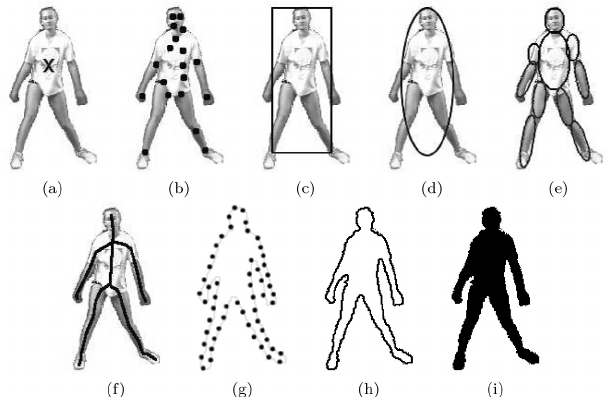
\includegraphics[width=0.8\textwidth]{figures/Object-representations.png}
  \caption{Different representations of objects. Credit: \cite{trackingsurvey}}\label{fig:objectrepresentation}
\end{figure}

\citeauthor{firstflow} \cite{firstflow} abstract the detected blob into a single point which has the largest distance to the background, and use this point as human body location. By tracking, the same label is assigned to a new blob if its distance to a previously seen blob is less than 10\% of frame width. In addition to the spatial constraint, the authors use a temperature feature to mark a blob, two blobs in sequential frames are considered the same person if their temperature difference is less than $1^\circ C$.

\citeauthor{mika} \cite{mika} also use the blob centroid to represent the human body location. Because the original resolution of the used IR camera is too coarse (only 8 by 8), they need to interpolate the image to $71\times71$ for tracking). Note that for a camera with $8\times8$ resolution, a spacial difference threshold of 10\% of the frame width is less than 1 pixel, which is impossible. Instead of matching the current position of a human body with a previously seen position directly, the authors smoothen the location updating with a Kalman filter \cite{kalmanfilter}. Similar tracking algorithms that are based on nearest neighbour association and Kalman filter can also be found in \cite{melexis,virtualtrack}.

By multiple blob association in one scene, a common challenge is to track merging/ splitting blobs correctly. When two people occur in the same frame, it is required that their blob representations have at least one pixel distance, otherwise the two blobs will be regarded as one large blob. Due to the low-resolution nature of IR-TAS, a gap of one pixel in the final image typically means some tens of centimeters between two people \cite{mika}. This issue is very hard to deal with in the tracking layer, which forbids tracking more than two people (because two people already amount to more than half of the camera view) or tracking any scenarios that two people may stand close, even for a short period of time.

An attempt to solve the issue is proposed by \cite{firstflow}. If one blob is large enough to be two merged blobs (larger than 30\% of frame's area), the background temperature threshold will be increased continuously at a step of $0.25^\circ C$ until a gap between two blobs emerges or the blob size shrinks to less than 10\% of frame area.

\citeauthor{virtualtrack} \cite{virtualtrack} try to solve the issue in the tracking layer. When two blobs merge, virtual trajectories will be created for both object with their previous positions and velocity. The merged human objects will be further propagated with their last seen velocity until the two blobs split. When the actual location points for both blobs are available again, the object position will be associated with an object label if it appears on the expected position given by a virtual trajectory. Since the positions in a virtual trajectory may deviate from the real ones significantly, the virtual trajectory will be replaced by a smoother back traced trajectory which connects the last actual position before merging and the first position after splitting. \autoref{fig:virtualpath} demonstrates the virtual trajectory tracking process.
\begin{figure}
  \centering
  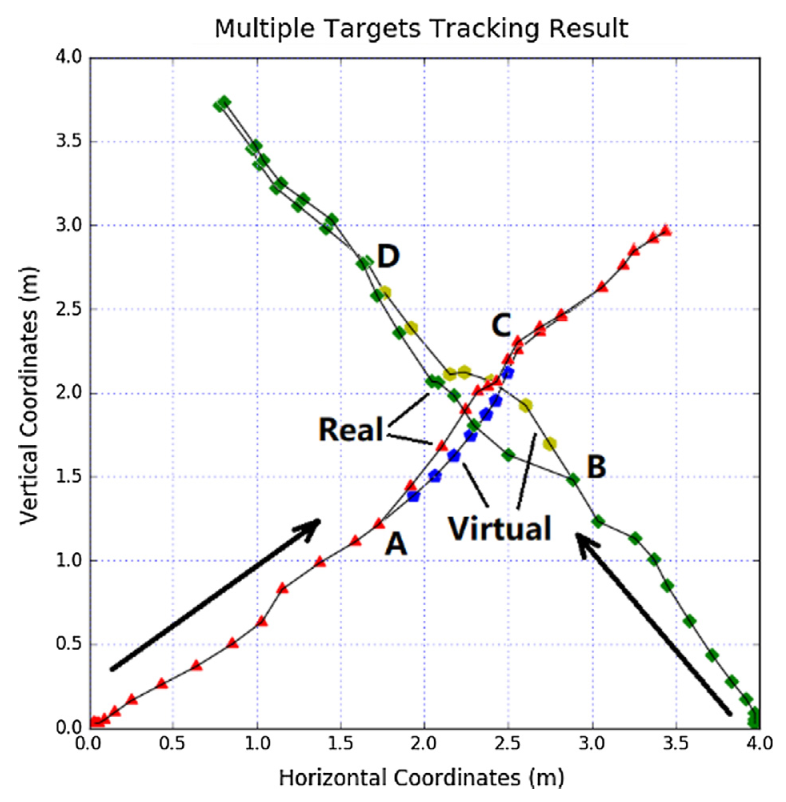
\includegraphics[width=0.5\textwidth]{figures/virtualpath.PNG}
  \caption{Multiple objects tracking result using virtual trajectory. Credit: \cite{virtualtrack}}\label{fig:virtualpath}
\end{figure}

Overall, we notice that a few related works have solved the aforementioned issue. We argue that two people moving in opposite direction through a doorway is a common scenario. Though people tend to keep a social distance of several tens of centimeters in a public space, at a narrow doorway they usually tilt the body to pass simultaneously rather than waiting the other to pass. Inevitably, the result of such a scenario will be a merged blob, which should be taken into consideration by the tracker's initial design.






\chapter{Problem Statement and Hardware Selection} \label{ch:hardware}
We want to develop a low-cost, easy to install doorway human counter device for room occupancy estimation. The main component of the device is a low-resolution thermal camera to guarantee privacy protection as well as detection of a static human. Relative counting is done by tracking the human object passing through the doorway and determine whether it is an entering or exiting event. Final occupancy estimation of a room could be obtained by accumulating all relative counts of a device, or several devices, in case of a room with multiple entrances. Moreover, the camera should be installed on the top of a doorframe or on the ceiling of a corridor, facing towards the ground. By this way the size of the monitored person is invariant with respect to the position in the frame, which cuts down the complexity of the tracking procedure.

The captured image frames should be sent to a microprocessor where the detector and tracker algorithms are implemented. When a frame sequence terminates and the relative count is obtained, this count value should be transferred to a data storage platform for further processing and long term storage. The data transfer should be wireless to ensure easy installation of the device. We want to keep the device design as simple as possible with minimal components. A Wifi-MCU (micro-controller unit) would be an ideal choice because no other radio components are needed.
\section{Infrared Camera}
For the IR-camera we have considered two candidates: the MLX90640 from melexis and the Amg8833 Grideye from Panasonic. The main attributes of both cameras are listed in \autoref{tab:ircameras}. Among all the technical features, a sufficiently high frame rate is essential so that the whole traversing event could be captured. When installed at a height of 2 meters, both cameras cover about 2.3m along the moving direction. If we subtract the border where a human is partially seen, the valid length left for tracking is merely about 1.7m. Assuming human walking speed is $1.4m/s$, a normal traverse event will last about 1 second. And at least 3 frames should be captured for a simple single-human event. More frames are required for a complex scenario. Overall a minimal frame rate of 8Hz should be reached.

The MLX90640 outperforms AMG8833 in accuracy and resolution. Though we are aware that a better camera may simplify the algorithm design drastically, the AMG8833 is chosen because of its low cost.
%TODO: Add agreement that the values where not stable und we head the lines.
\begin{table}[]
\caption{Comparison of the MLX90640 and AMG8833}\label{tab:ircameras}
\centering
\begin{tabular}{lll}
                                      & MLX90640                                      & AMG8833                  \\ \hline
\multicolumn{1}{l|}{resolution}       & \multicolumn{1}{l|}{32$\times$24}             & 8$\times$8               \\
\multicolumn{1}{l|}{frame rate}       & \multicolumn{1}{l|}{0.5$\sim$64 Hz}           & 1 or 10 Hz               \\
\multicolumn{1}{l|}{FOV}              & \multicolumn{1}{l|}{$55^\circ\times35^\circ$} & $60^\circ\times60^\circ$ \\
\multicolumn{1}{l|}{measuring accuracy} & \multicolumn{1}{l|}{$\pm 1^\circ C$}        & $\pm 2.5^\circ C$        \\
\multicolumn{1}{l|}{interface}        & \multicolumn{1}{l|}{I2C}                      & I2C                      \\
\multicolumn{1}{l|}{cost}             & \multicolumn{1}{l|}{€60}                      & €20
\end{tabular}
\end{table}

The hardware limits of the AMG8833 have been discussed by many researchers.
\begin{itemize}
  \item high sensor noise: the product datasheet states that the worst case temperature difference between two pixels is $5^\circ C$ even if the camera faces towards a homogenous temperature surface \cite{grideye_datasheet}. This significant noise level is further confirmed by a experiment \cite{firstflow}.
  \item short detection range: IR waves emitted by human body characterize an amplitude drop as the distance increases. But the reading of AMG8833 drops more faster than other high-end alternatives. At a distance of 120cm, the measurement of a human body is around $18^\circ C$, which is approximate to the room temperature \cite{firstflow}.
  \item radial distortion: the pixel detection areas are not evenly distributed as a $8\times8$ grid, see \autoref{fig:grideyedetectionarea}. The barrel distortion could be fixed by applying Brown's lens correction (\autoref{eq:brownscorrection}), where $r_c$ and $r_u$ are corrected and uncorrected distance to the optical axis. The reported radial coefficients are $K_1=7.4\times 10^{-3}$ and $K_2=0.17\times10^{-3}$ \cite{gonzalez2013using}.
\end{itemize}
\begin{figure}
  \centering
  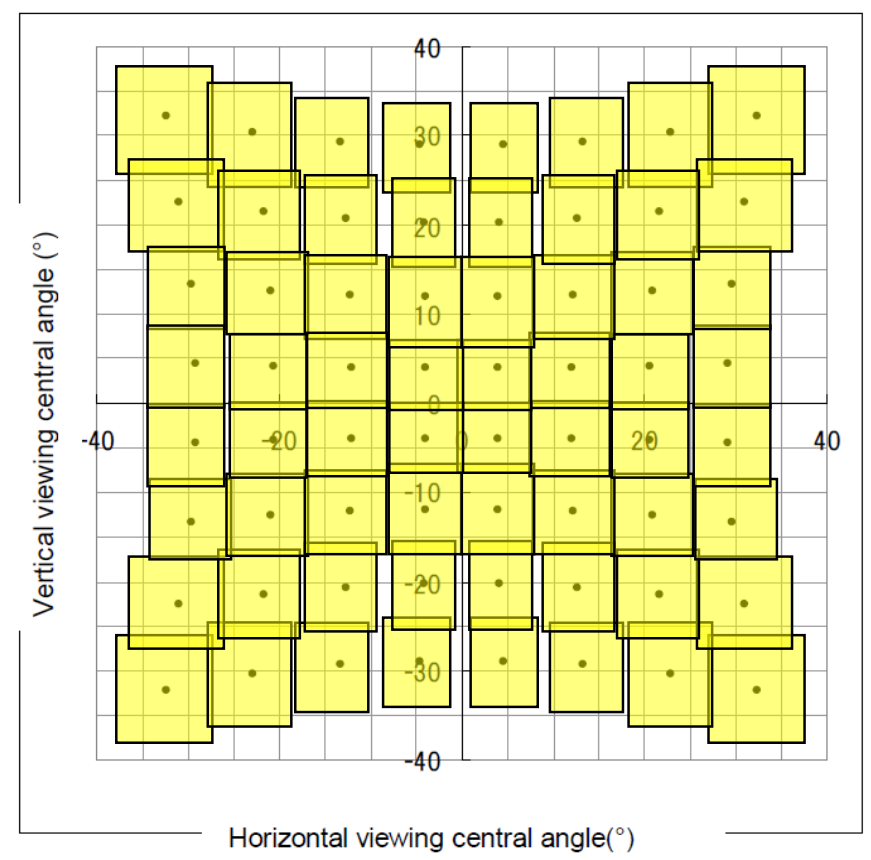
\includegraphics[width=0.6\textwidth]{figures/grideye_detectionarea.PNG}
  \caption{Detection area of each pixels of the Grideye sensor. Credit: \cite{grideye_datasheet}}\label{fig:grideyedetectionarea}
\end{figure}
\begin{equation}\label{eq:brownscorrection}
  r_c = r_u + K_1r_u^3+K_2r_u^5
\end{equation}
\section{Temperature Sensor}
The AMG8833 comes along with a on-board thermistor which measures its working temperature. \citeauthor{trofimova2017indoor} \cite{trofimova2017indoor} estimate the ambient temperature with the thermistor reading because they have a linear dependence. Nevertheless, an external temperature sensor that reads the accurate room temperature is useful, especially in case the IR module malfunctions.

We have chosen a DHT11 temperature and humidity sensor \cite{dht11} for this purpose. It measures the surrounding temperature at $1^\circ C$ precision.
\section{Main Processor}
The microprocessor should have one I2C interface to retrieve data from the IR camera. Since a new frame must be read every 0.1 second otherwise it will be covered by following frames, a realtime task support is required. The MCU should have a on-board radio component to send out data without an edge device. In addition, we want to store the frame sequences for debugging and let the tracker replay them frame by frame, an UART interface is required to simulate the camera frame input.

Our choice for the main processor is a ESP32-WROVER module from Espressif \cite{esp32wroverboard}. The specifications are shown in \autoref{tab:esp32wrover}.

The ESP32 board contains not merely a microprocessor, but also a set of out-of-box development firmware such as Wifi and bluetooth protocol, see \autoref{fig:ESP32diagram}. The board could be run as bare metal, however, the ESP-IDF (Espressif Internet-of-things Development Framework) empowers it to run on an adapted version of FreeRTOS \cite{esp32freertos}. In a RTOS (real-time operating system), each logically independent code snippet could be encapsulated as a task. The RTOS task scheduler divides CPU process time to tiny time slices (1 millisecond), and always assign a time slice to the task with the highest priority in the ready list at that moment. A task will be blocked if it requires a resource that is not available, and it will not participate in task scheduling until the required resource is available again. By this way, a strong realtime response performance is largely guaranteed, unless the processor's maximum computation power is exceeded.

The ESP32-WROVER module features a dual-core architecture. It contains two Xtensa CPUs \cite{xtensa} with a frequency up to 240MHz. Wireless communication through Wifi or BLE is inherently handled by the first core, while user applications could be attached to either core. The powerful computational capacity and its low cost (€10) made it our first choice for the main processor.
\begin{table}
  \centering
\begin{tabular}{l|ll}
                & ESP32-WROVER     & Required \\ \hline
I2C interface   & 2                & 1        \\
UART interface  & 3                & 1        \\
GPIO pins       & \textgreater{}10 & 1        \\
realtime task   & FreeRTOS         & yes      \\
radio component & Wifi, bluetooth  & yes      \\
flash           & 4MB              & -        \\
RAM             & 520KB            & -
\end{tabular}
  \caption{Specifications of the ESP32-WROVER module}\label{tab:esp32wrover}
\end{table}
\begin{figure}
  \centering
  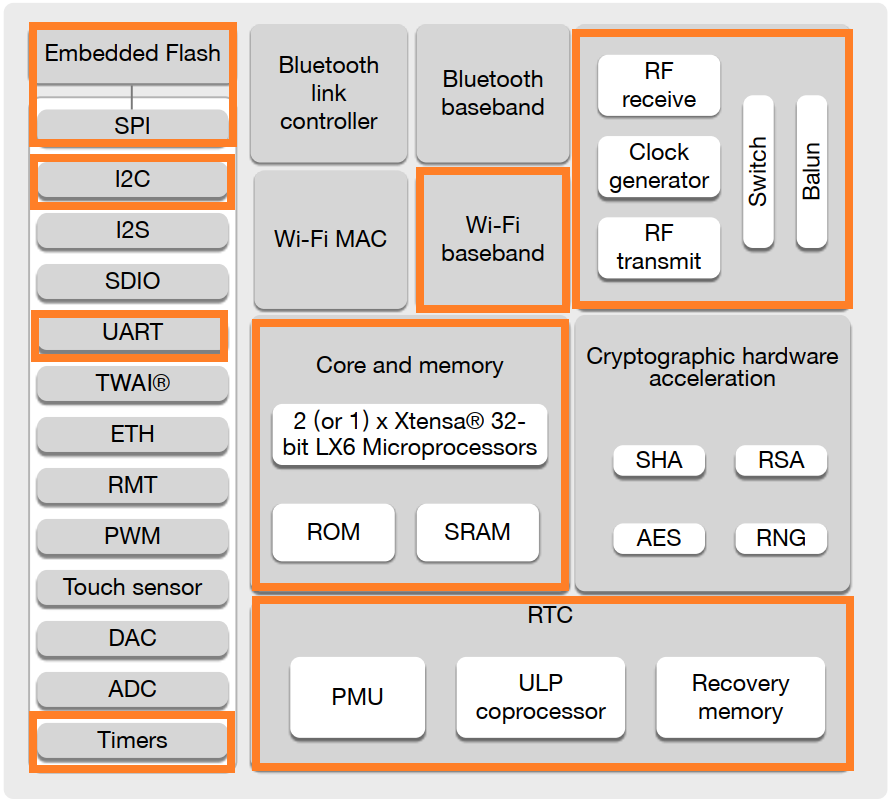
\includegraphics[width=0.5\textwidth]{figures/ESP32diagram.PNG}
  \caption{Functional block diagram of ESP32 chip. The circumscribed modules are used in out application.}\label{fig:ESP32diagram}
\end{figure}


The total cost of our design is €35, including an AMG8833 Grideye (€20), an ESP32 board (€10) and a DHT11 temperature sensor (€5).


\chapter{Data Transmitting and Platforms} \label{ch:platform}
The statistic data collected by a doorway counter is not of much use until it is analyzed. For a quick acquisition of data and a frequently updated overview of the room occupancy, the count value should be immediately sent to a remote platform for further visualization and analysis.
\section{MQTT protocol}
We use MQTT (message queuing telemetry transport) to transfer data because it is supported by the ESP-IDF and widely accepted in IoT use cases. MQTT is an application layer protocol built on top of Wifi and TCP/IP. It is a light-weight, publish-subscribe network protocol, its structure is shown in \autoref{fig:mqtt}. When a publisher publishes, instead of sending to the receiver directly, the message is sent to a intermediate server called broker. Each message is published to a specific topic, a client would filter the messages by the subscribed topic and could only receive the message if it is listening to the same topic.

The light-weight usage of MQTT is mainly reflected by its transparent topic mechanism. A client does not need to create a topic before it publish or subscribe to it. A topic keeps alive when there is at least one publisher or subscriber. When a topic has at least one client on both pub/sub side, the data transmission becomes valid almost immediately. The topics in MQTT decouple the rigid connection between clients, reducing the complexity of connection drastically regardless of the scale (up to tens of thousands per MQTT server).

The main drawback of MQTT is no message buffering. A QoS (Quality of Service) setting higher than 0 on the client side only confirms that the message is received by the broker. If a message is published to a topic without listeners, that message is lost forever. Latest versions of MQTT supports retained messages, which stores one \emph{last known good value} in the broker. However, the retained messages aim to serve as a \emph{initialization default value} for those subscriber that join the topic between two publish intervals, storing more than one message is impossible.
%事实错误:Secondly, MQTT is a queuing system instead of streaming, it delivers messages to a single consumer. When there are multiple consumers subscribing to a topic, they will consume the messages in a round-robin manner.
\begin{figure}
  \centering
  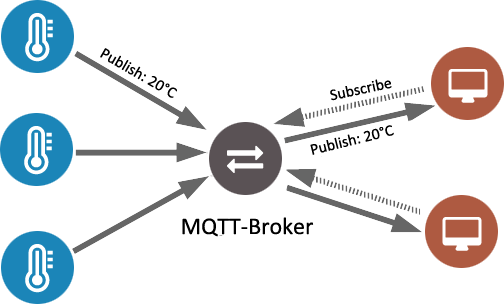
\includegraphics[width=0.6\textwidth]{figures/mqtt.png}
  \caption{MQTT network structure}\label{fig:mqtt}
\end{figure}
\section{Node-Red}
Visualization of an image frame sequence on websites often requires extensive programming. Fortunately, Node-Red \cite{nodered} relieves us from irrelevant affairs so that we can concentrate on the doorway counter development. Node-Red is a web-based visual programming editor that connects IoT devices or acts as an end-consumer. It supports message input from a MQTT broker, as well as http, websocket and serial. The smallest execution unit is called a node. A complete data process procedure consists of multiple nodes and is called a ``flow'', an example is shown in \autoref{fig:noderedflow}. Messages are propagated from flow start to flow end, and could be modified, truncated, merged with other flows, or splitted.
\begin{figure}
  \centering
  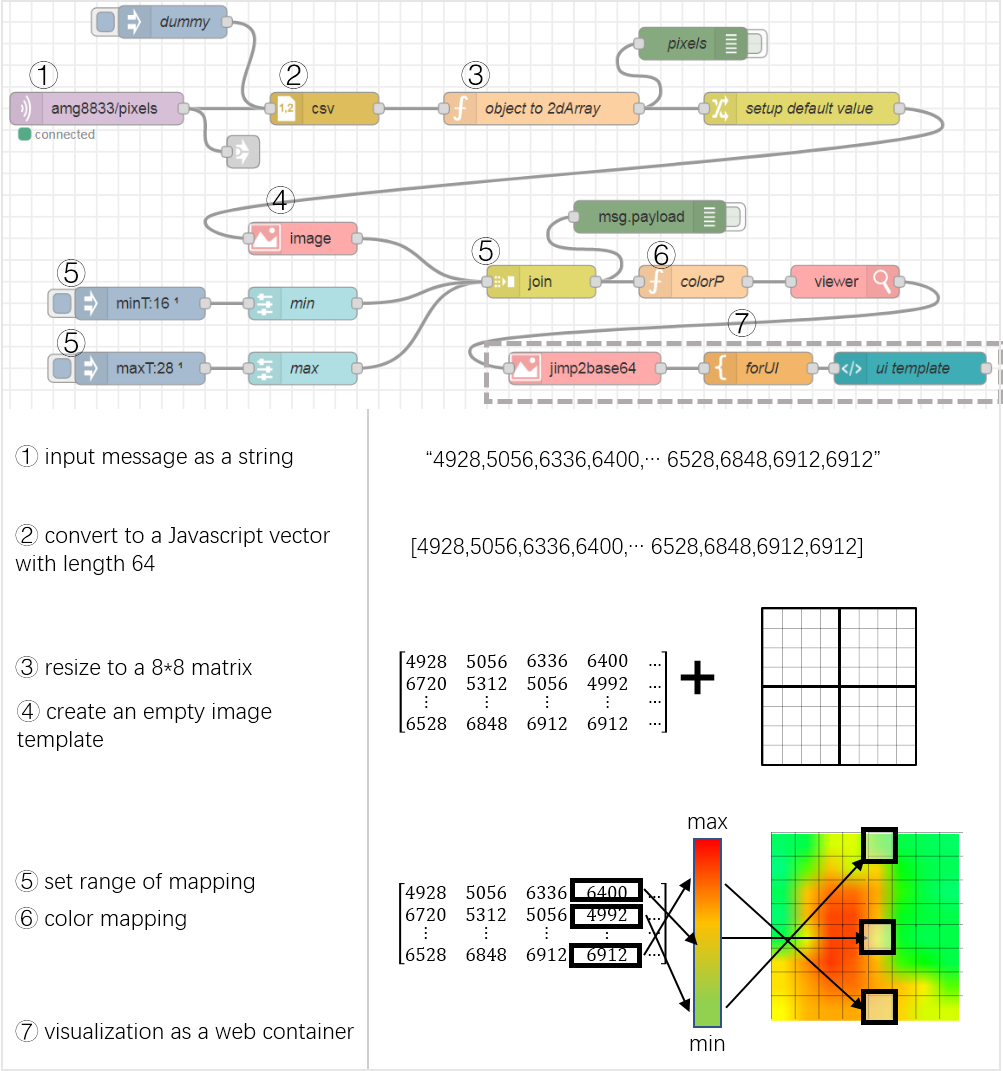
\includegraphics[width=0.8\textwidth]{figures/noderedflow.PNG}
  \caption{Our Node-Red flow used for $8\times8$ pixels image visualization}\label{fig:noderedflow}
\end{figure}
\begin{figure}
  \centering
  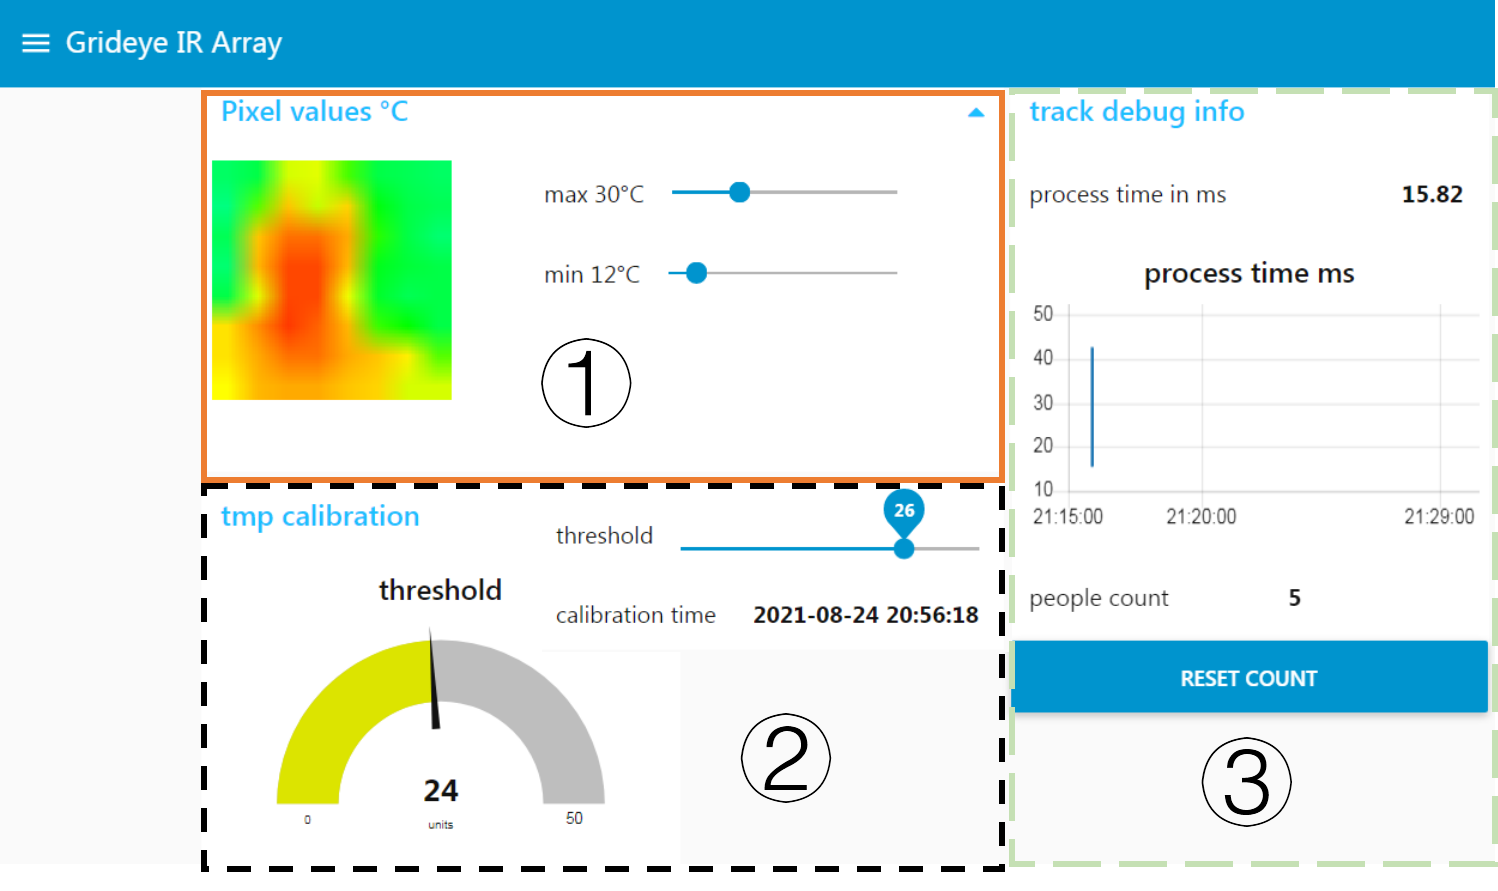
\includegraphics[width=0.8\textwidth]{figures/noderedui.png}
  \caption{Our NodeRed visualization panel is divided into three sections: (1)raw image frame, (2)temperature sensor reading, (3)debug info}\label{fig:noderedui}
\end{figure}

Node-Red has integrated a dashboard which could be used for data visualization. Data in a simple format like an integer number or a string, can be visualized with offered presets with no effort. Complicated data like images can be visualized with custom javascript and Angular framework scripts. \autoref{fig:noderedui} shows the dashboard used in our project. The dashboard contains three subsections: region 1 on top-left shows the actual camera view, grayscale pixel values of the IR camera are converted to a heat map, where redder pixels represents a hotter temperature; region 2 shows the last updated room temperature given by the temperature sensor, which is used for camera calibration, and this value could also be manually assigned; region 3 shows the process time of a single frame and the actual count number, the former is crucial to check whether our algorithm could meet the frame rate constraint, the latter is useful to get an immediate feedback whether the algorithm works properly when we witness an enter or exit event in region 1.

Node-Red has a ``file'' node which terminates the flow and stores messages on local storage. We store image files by this way to bypass the MQTT's buffering issue. We don't store images in a database because the generated images accumulates to 70MB every day.
%todo: overview of network dataflow
%
\section{ElasticSearch and Kibana}
To evaluate whether our algorithm outputs the expected relative count, a long-term storage of the count value is needed. For this purpose a data bank based on ElasticSearch and Kibana is used. In ElasticSearch, an individual message is called a ``document'', and a series documents that are similar or generated by a same source are gathered in a group called ``index''. Kibana is a visualization tool combined with ElasticSeearch that can visualize data by indexes. Developed by TUM researchers, the IoT platform we used has an MQTT interface which receives time-series data, and the accepted message format is one float number and a timestamp.

In our use case, whenever an enter or exit event is detected, a pair of messages, the actual timestamp and the count value at that time will be published and recorded in the database. \autoref{fig:ESKibana} shows the recorded data in one afternoon, where the green line is the output of the counting algorithm and the red dots are the ground truth, annotated manually by watching the stored image sequence. Details about ground truth annotation and the evaluation result will be elaborated in \Cref{ch:evaluation}.
\begin{figure}
  \centering
  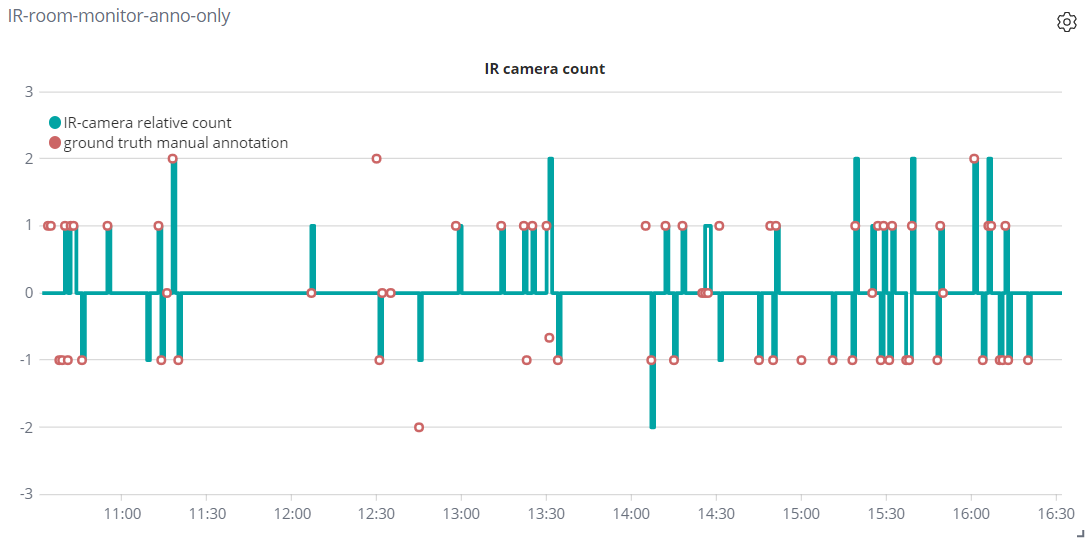
\includegraphics[width=0.8\textwidth]{figures/ESKibana_overview.PNG}
  \caption{A fraction of the recorded data. Green line shows the output of the algorithm and red dots are the ground truth.}\label{fig:ESKibana}
\end{figure}



\chapter{Proposed Algorithm}\label{ch:algorithm}
The objective of the human counting algorithm is clarified as following.

The detector should be capable of detecting human objects in a relative large range of temperature, because the detected temperature of human body depends heavily on the wearing clothes and individual body condition. The detector should be sensitive to detect a human that is slightly hotter than the ambient environment. Meanwhile, fluctuation of the environment temperature should be taken into account carefully. A pixel value that is just above the ambient temperature in a cool morning would be regarded as active, but the same value would probably be a noise reading in the afternoon of the same day.

The human body tracker should work properly for single human events, as well as more complicated events when multiple people interact with the door, including but not limited to: two people traversing parallel, traversing sequential but with a narrow distance, traversing in opposite direction, or one person standing still and another pass by. The tracker should not assume that the detected pixel blobs are separated perfectly, and should be able to track two once separate blobs when they merge, as well as assign the correct labels when they split again.

And finally, the time consumption of one single image processing must be constraint within 100ms because the camera runs at 10fps. Considering that other tasks, such as data reading from camera register and publishing MQTT messages, also takes CPU process time, the time window left for detecting and tracking is merely around 50ms.

An overview of the algorithm is shown in \autoref{fig:algorithm_diagram}.
\begin{figure}
  \centering
  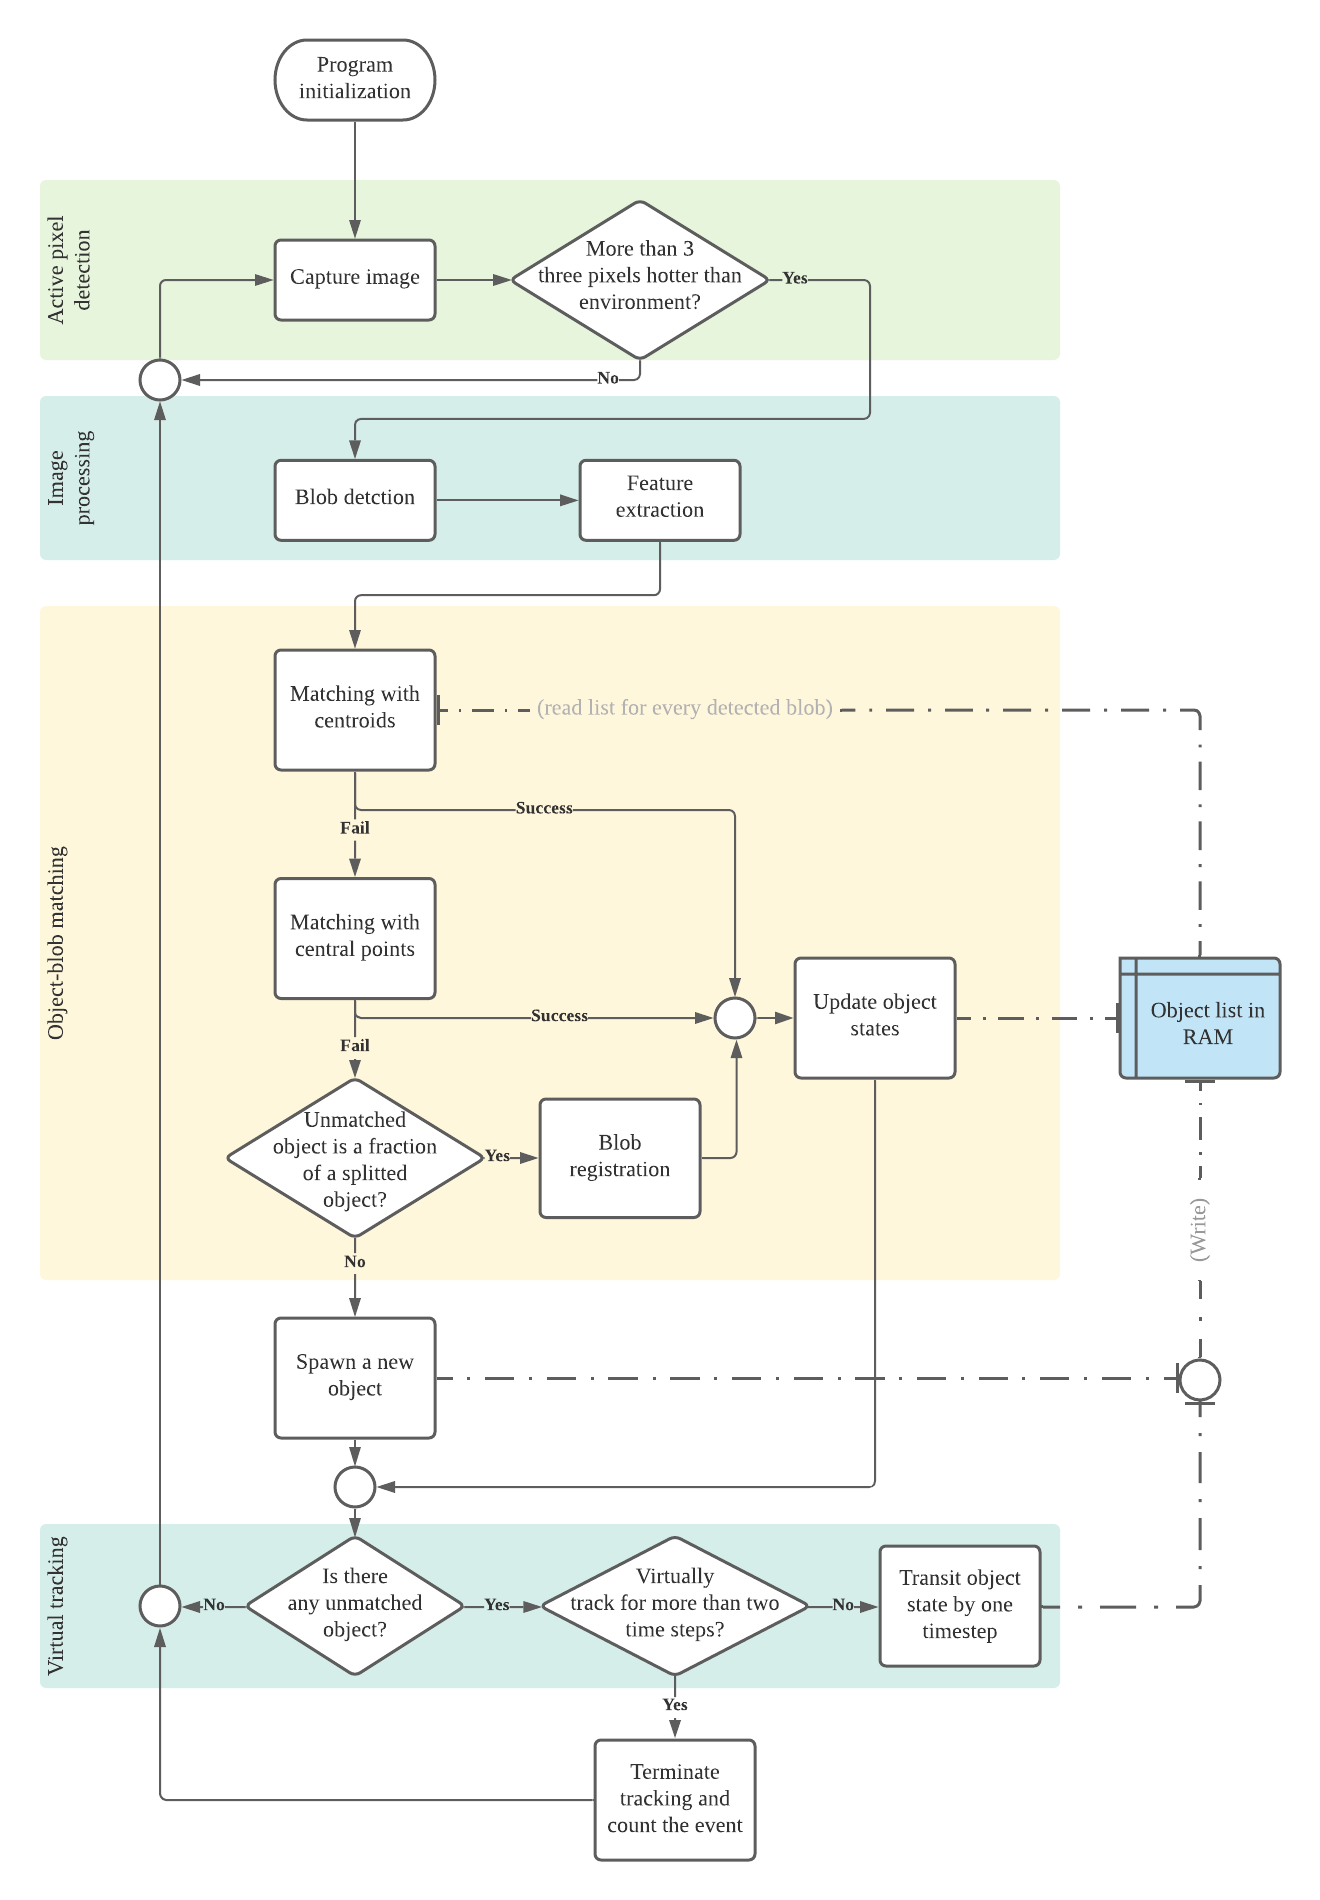
\includegraphics[width=0.8\textwidth]{figures/Program_block_diagram.png}
  \caption{An overview of the proposed algorithm.}\label{fig:algorithm_diagram}
\end{figure}

\section{Blob Detection} \label{sec:detect}
\subsection{Active Pixel Detection}
Before the actual fore- and background segmentation, an early detection process is conducted on the $8\times8$ coarse image to see whether there is a potential heat source in the camera view. We check if there are at least three pixels having a value $1.5^\circ C$ higher than the room temperature. The parameters are chosen based on the following calculation. When installed at a height of $2.5m$, the Grideye sensor covers an area of about $8m^2$, which is much larger than a human body. However, when a human enters the camera view, the projection of his body on the image is caused by the horizontal plane of the shoulders, which is much higher than the ground and closer to the camera. Assuming the average shoulder height is $1.4m$, the real coverage of the camera is $4m^2$, only half of the ground area that it can cover. We assume the horizontal plane of a human body is not less than $2dm^2$, which amounts to at least three pixels in the image frame. The threshold $1.5^\circ C$ above the room temperature is chosen to filter out the sensor noise, we denote this threshold as $T_{lb}$ (low boundary).
%todo: 大概的示意图
\subsection{Segmentation Threshold Determination}
To separate human objects from the background, we follow the idea of calculating a global threshold from image statistic values, which is inspired by \cite{virtualtrack} and \cite{jeong2014probabilistic}. The threshold $T_{th}$ is calculated by the following formula (\autoref{eq:detectionthreshold}), where Max is the maximum pixel value among all 64 pixels and SD is the standard deviation. By thresholding, the original raster image is linearly interpolated to a resolution of $71\times71$ by inserting nine pixels between each pixel to avoid numeric issues in the following segmentation. The same resolution is also used by \cite{virtualtrack} and \cite{mika}.
\begin{equation}\label{eq:detectionthreshold}
  T_{th} = max\{Max - 4\times SD, T_{lb}\}
\end{equation}

The formula is simple but effective. The result is shown in \autoref{fig:detectioninterpolate}. Comparing image (c) and (e), it is apparent that the interpolation step is necessary to preserve more information from the original image and obtain a smooth shape of the object.
\begin{figure}
  \centering
  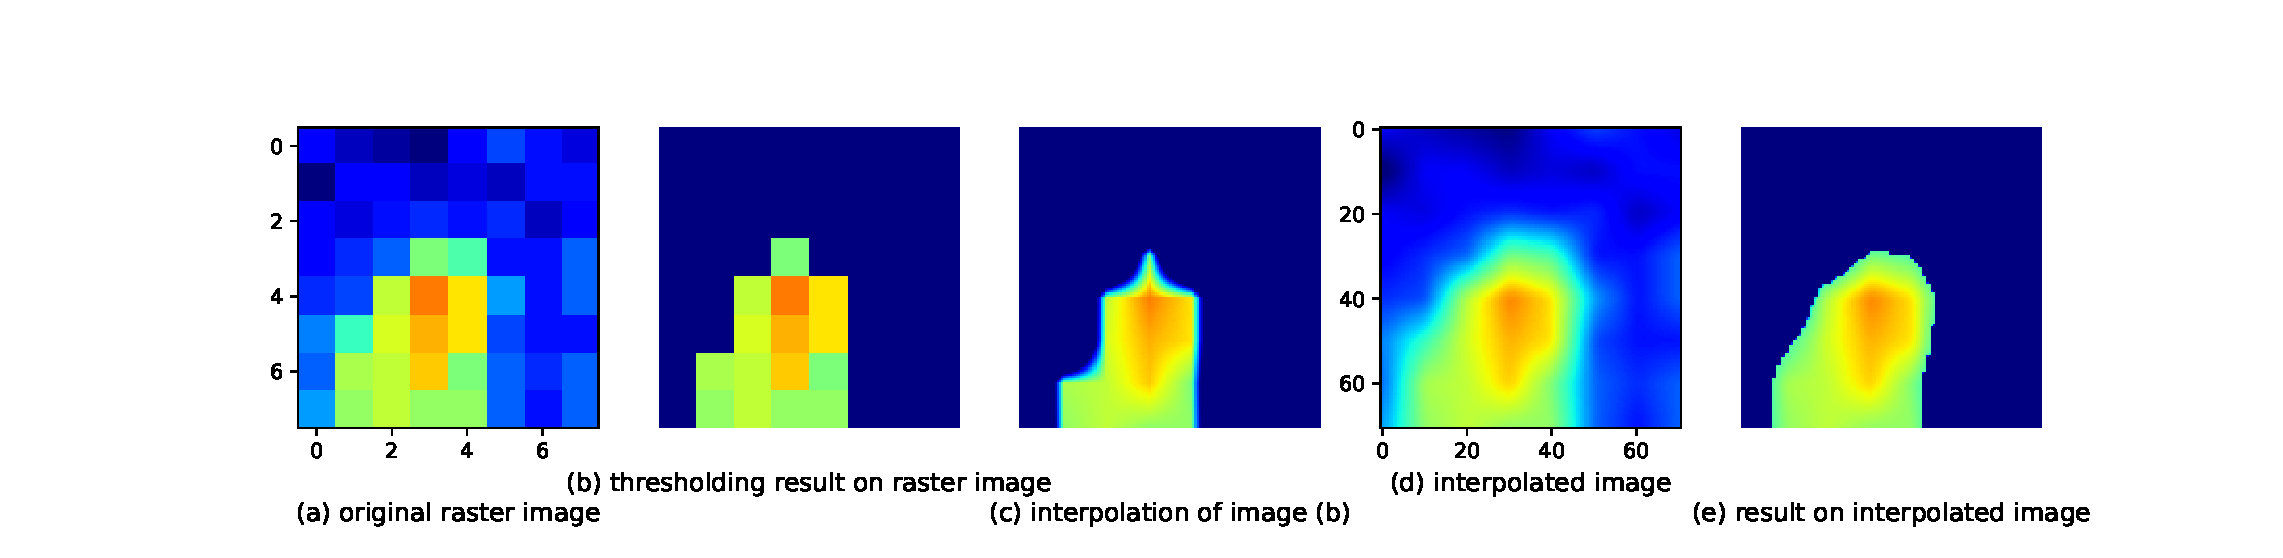
\includegraphics[width=\textwidth]{figures/detect_interpolate.eps}
  \caption{Result given by \autoref{eq:detectionthreshold}, the interpolated image preserves more details after thresholding.}\label{fig:detectioninterpolate}
\end{figure}

\subsection{Spacial Active Pixel Filter}
We notice that a single global threshold cannot separate two close objects very well. When two human stand close to each other, the small region between them will have a temperature higher than the room temperature because the pixel value results from a size-weighted average of both objects and background. This effect creates fake active pixels in the binary mask, see the first row in \autoref{fig:detectionspatialfilter}.

Therefore, pixels higher than the threshold but with hotter pixels nearby should be ignored because they originates from those hotter pixels and do not represent the true heat distribution. Reversely speaking, only those pixels that are hotter than its surrounding, namely local maxima pixels, contain valid information. We use the average filtered image as a spatial filter. After experiments on the collected image frames, a kernel size of 36 is chosen (half of the frame width). The value of every pixel in the filter is calculated by averaging a $36\times36$ neighbourhood surrounding that pixel location in the original image. Afterwards, the original image is compared with the filter pixel-wise, and only those pixels with a value higher than its filter counterpart will be kept. \autoref{fig:detection3d} shows the process in a surface plot, it shows the same image frame from \autoref{fig:detectionspatialfilter}. The threshold calculated from \autoref{eq:detectionthreshold} is applied to the local maxima image. The result is shown in the second row of \autoref{fig:detectionspatialfilter}, it is clear that the bridge connecting two objects becomes much narrower, which is beneficial for recognition as there are two objects in the frame, instead of one single large object. Moreover, it is not necessary to eliminate the bridge completely as we have a feature extraction step, which will be discussed in the next section.
\begin{figure}
  \centering
  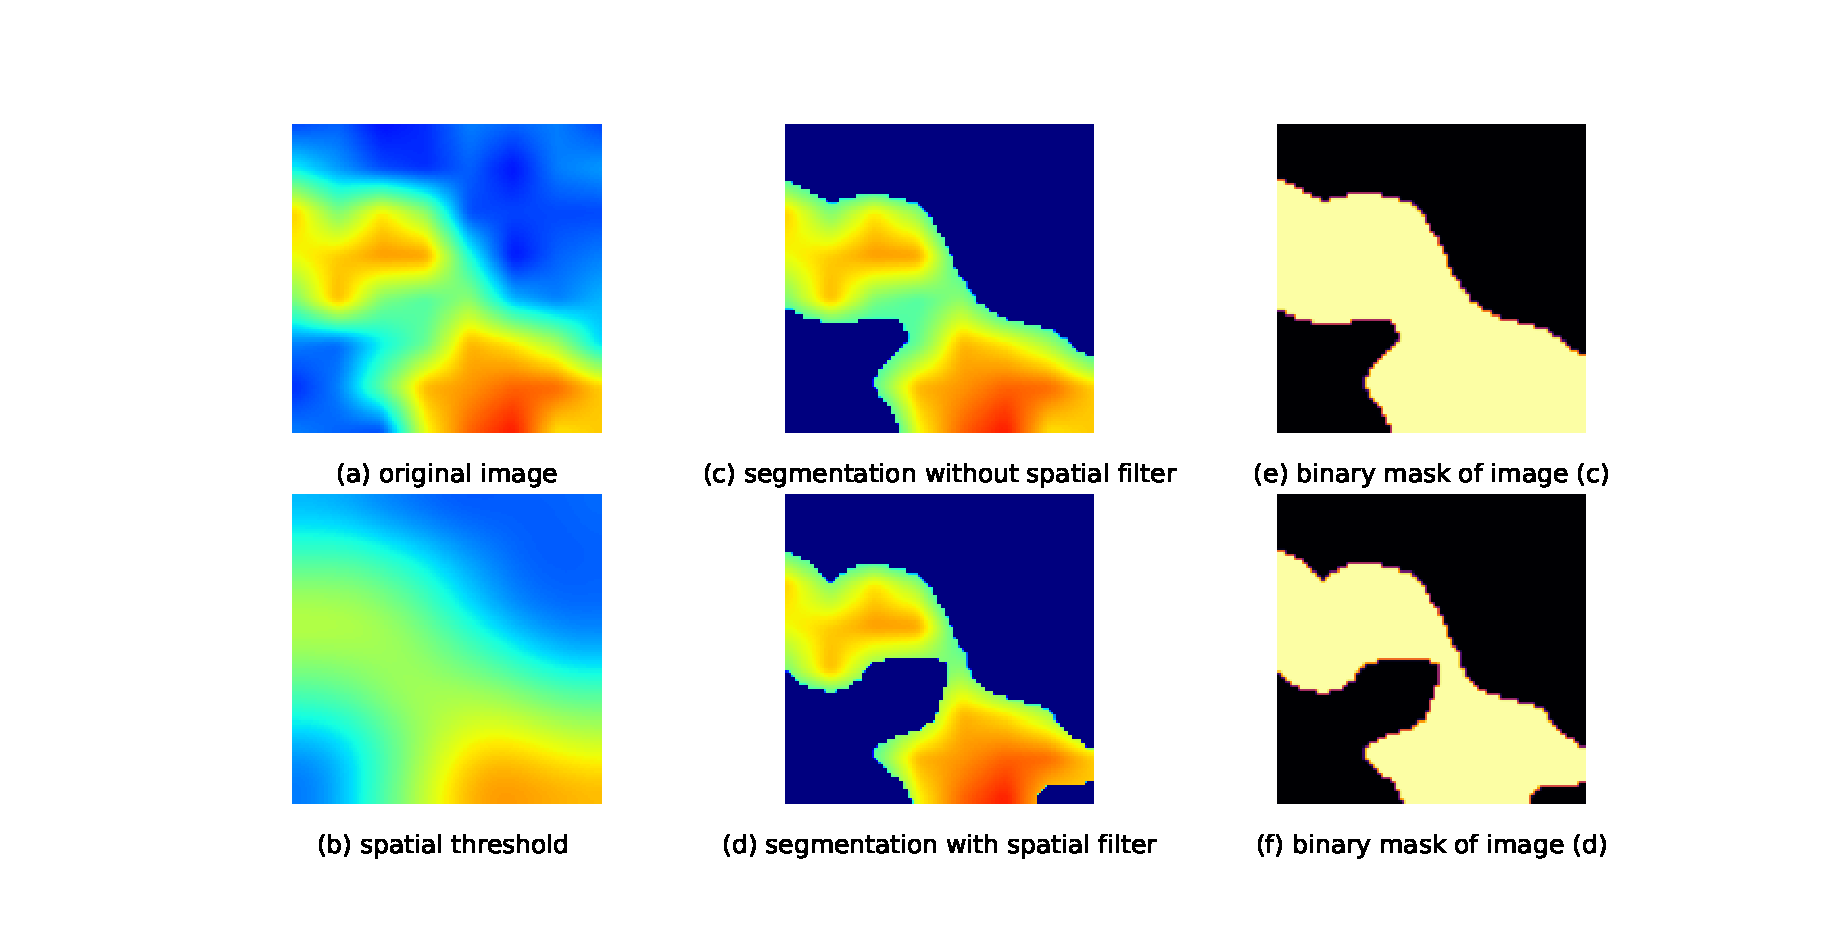
\includegraphics[width=\textwidth]{figures/detect_spatialfilter.eps}
  \caption{After introducing a spatial filter, the region between two objects are no longer marked as occupied.}\label{fig:detectionspatialfilter}
\end{figure}
\begin{figure}
  \centering
  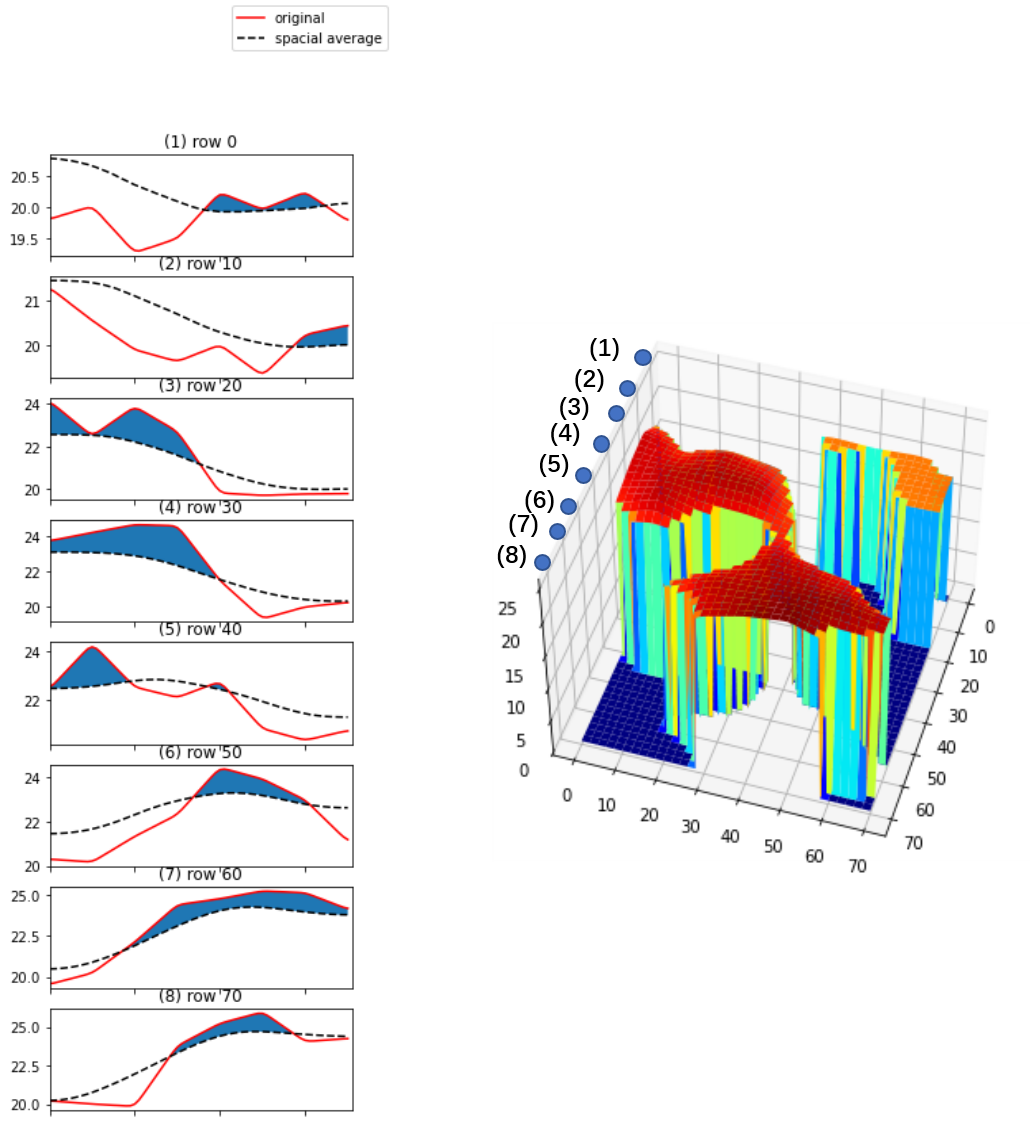
\includegraphics[width=\textwidth]{figures/spacefilter.png}
  \caption{The spacial average filter only keeps those pixels hotter than the region average.}\label{fig:detection3d}
\end{figure}

Moreover, this method outperforms simply increasing the global threshold because it has a better generalization ability for different body temperature. Though the aforementioned pixel bridge could also be eliminated by increasing the global threshold, we find that the threshold must be set very high to obtain a similar result. \autoref{fig:detectioncompare} shows the result of both method in two real scenarios. The first row shows the same frame in \autoref{fig:detectionspatialfilter}, where a tight global threshold of $Max-1.5\times SD$ turns out to be even better than our proposed method. However, when two human with distinct temperature occur in the same frame, the hotter object raises the global threshold with a higher $Max$ pixel value. The threshold will be too high for the cooler object, and only the hotter object is detected.
\begin{figure}
  \centering
  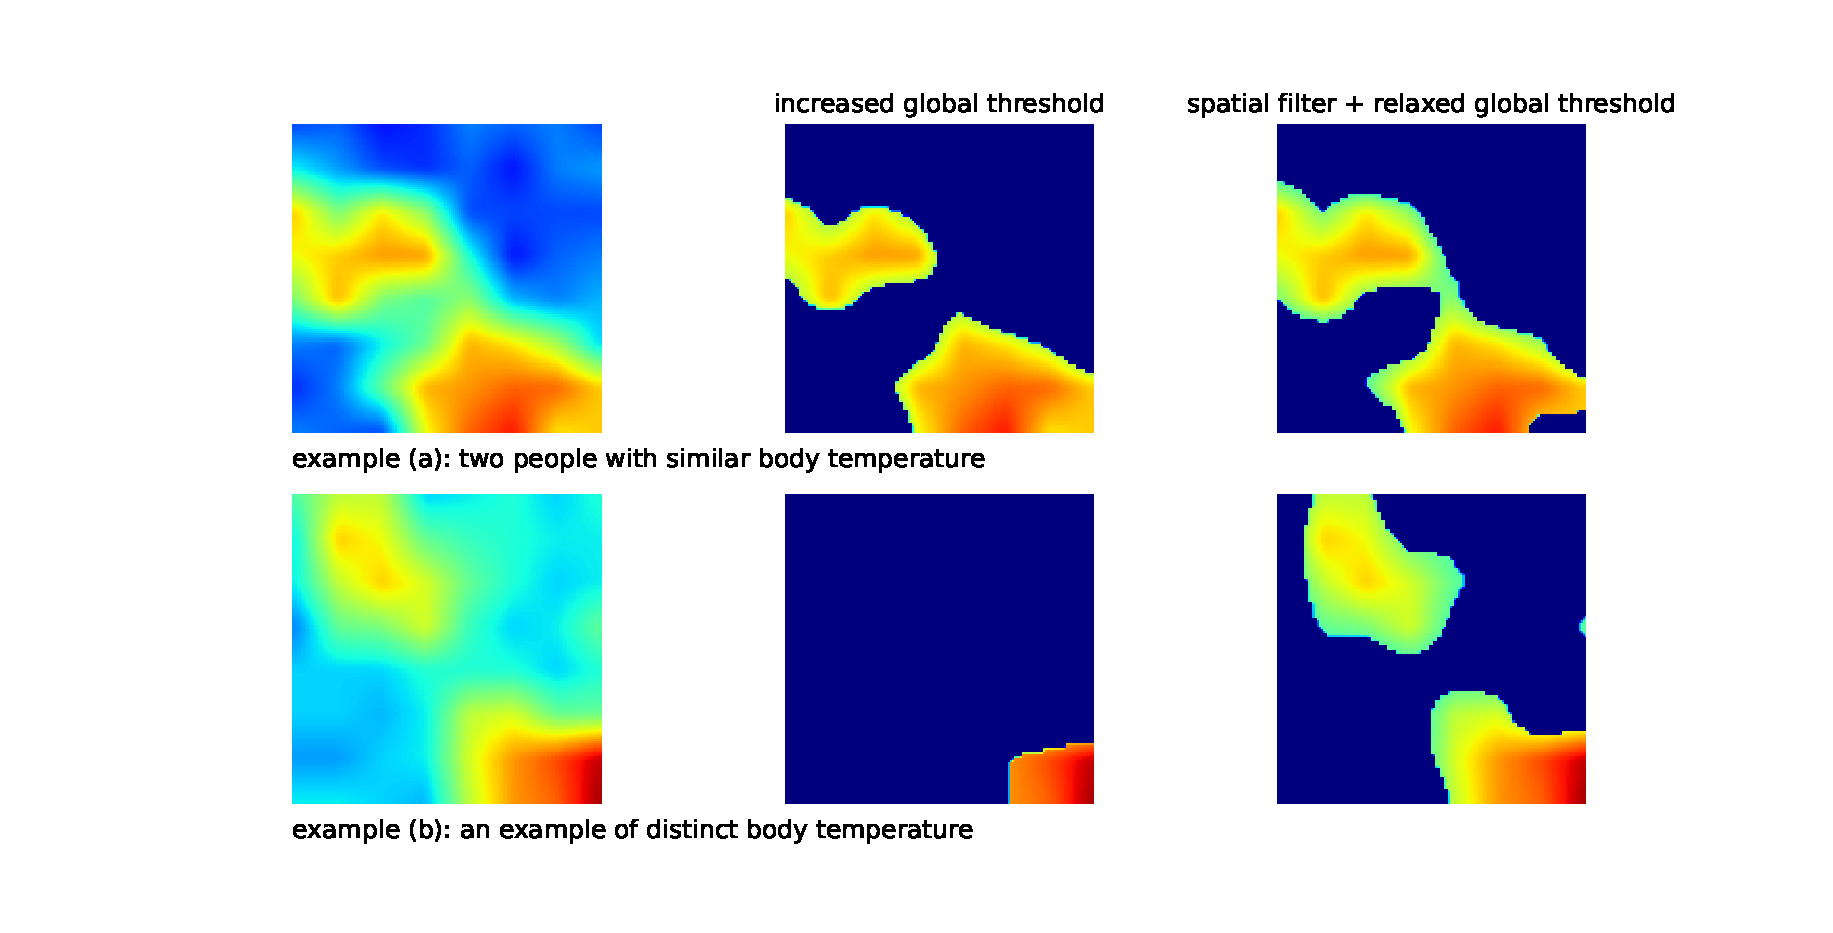
\includegraphics[width=\textwidth]{figures/detect_compare.eps}
  \caption{The middle column shows the segmentation result by a global threshold of $Max-1.5\times SD$, the right column shows the result by the proposed method. Both objects are detected whether they have distinct body temperature.}\label{fig:detectioncompare}
\end{figure}

With respect to the implementation, a convolution kernel with size $36\times36$ is too slow to meet the demand of realtime performance. For a $M\times N$ image and a $K\times K$ kernel, the time complexity of average pooling is $M\cdot N\cdot K^2$. Though the time complexity could be reduce to $M\cdot N\cdot K$ by separating the 2-dimensional kernel to two $36\times 1$ 1-dimensional kernels, the time consumption is still not satisfying. Our experiments show that on a ESP32 processor with 160MHz frequency, it takes seconds to convolve with a 2d kernel and about 70 milliseconds to convolve with two 1d kernels. We boost the processing performance by replacing the average polling algorithm with a summed-area table \cite{summedareatables}, which reduce the time complexity to $M\cdot N$.

A summed-area table, or sometimes called an integral image, is an image with the same size of the original image, where every pixel's value is the summation of all the pixels on the top-left of it. A summed-area table could be calculated efficiently from the original image in a recursive way, because the value of each pixel only depends on three pixels above, on the left and on the left-top of it.
To calculate the average value of a sub-region in the original image, only four corner points of that region in the summed-area table are needed. \autoref{fig:summedareatable} demonstrates how a summed-area table is calculated and used.

\begin{figure}
  \centering
  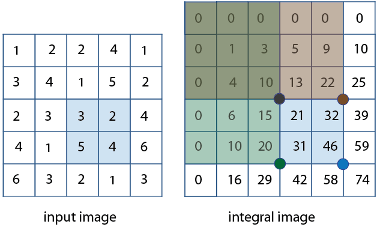
\includegraphics[width=0.6\textwidth]{figures/summedareatable.png}
  \caption{The basic idea of a summed-area table. Credit: \cite{summedareatableimage}}\label{fig:summedareatable}
\end{figure}


For comparison, the summed-area table based average filter takes only around 2ms for a single frame with the same processor configuration.
\subsection{Hole Filling}
Another common issue in segmentation is caused by the hair isolation of the head. From a top view, the human body is typically represented as an ellipse containing the head, two shoulders and partial upper torso. Ideally, the blob representation should have the highest temperature at the center and have a descent gradient to the margin. Unfortunately, a lower temperature is often observed in the blob center because a person's hair decays the heat emissivity. This will create a hole in the final binary blob and cause confusion, see \autoref{fig:detectionhole}.
\begin{figure}
  \centering
  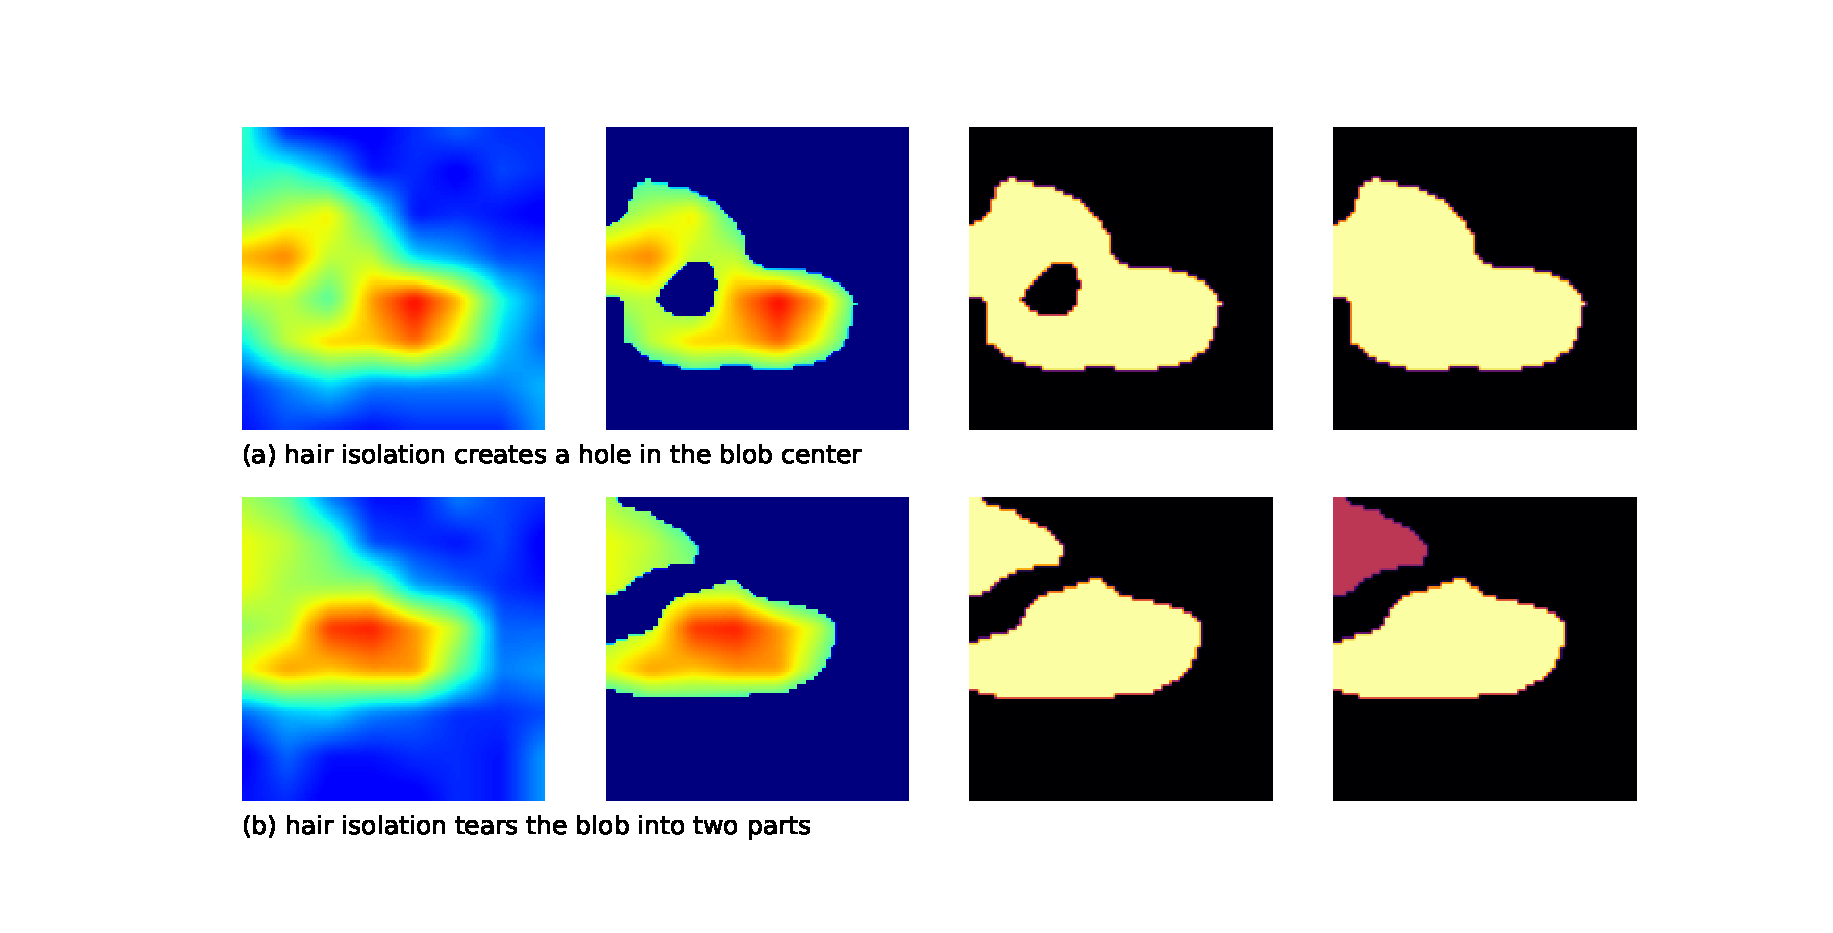
\includegraphics[width=\textwidth]{figures/detect_hole.eps}
  \caption{Two incorrect detection caused by hair isolation. The former could be fixed in detection layer, but the latter is left for tracking layer.}\label{fig:detectionhole}
\end{figure}

Since our detection method does not include any prior knowledge about the blob shape, any pixel that is cooler than the threshold will be regarded as background. There is no way to distinguish whether a pixel is truly a background pixel or belongs to a human but isolated. Moreover, because the hair is closer to the camera and has a large proportion in the blob presentation, the isolated region could be very large and even deteriorate the detection result.

If the hair isolation only creates a hole and the binary blob is still a connected domain, the hole could be filled with the flood-fill algorithm. Starting from the top-left pixel of the image, every connected background pixel is marked as occupied until there is no connected background pixel anymore. When there is a hole in the blob, the hole pixels are the only background left because they are surrounded by occupied pixels and are not reachable from a border background pixel. Then the processed binary mask will be logically reversed and merged with the original image. The final result is a blob representation without holes.

Nevertheless, if the hair isolation region is too large, the original blob will be separated into two parts, see the second row in \autoref{fig:detectionhole}. In this situation, even a human observer cannot distinguish whether it is a large person or two smaller people standing close by watching a single frame. A conclusion can only be drawn by taking previous frames into account. We decide not to solve this issue in the detection layer and leave it for the tracking layer. 
\section{Feature Extraction} \label{sec:featureextract}
The binary blob mask of an object contains too much redundant information for the tracking algorithm. As reviewed in \autoref{ch:review}, a binary blob could be represented as a feature vector of the centroid and the size, denoted as \autoref{eq:blobdenote1}, where $C$ is the 2D coordinate of the geometry center and $S$ is the total pixel number of the blob.
\begin{equation}\label{eq:blobdenote1}
  B = \{C,S\}
\end{equation}

This basic representation is sufficient for a single object tracking because the centroid is a unique feature for a blob. However, when two objects overlap and their blob masks merge together, they will be regarded as one single blob and therefore have only one shared centroid. The uniqueness of the centroid no longer holds, and the one-to-one matching relation between an object and its corresponding blob mask is broken.
\autoref{fig:blobmerge} shows an example demonstrating how the merged blobs impede the feature extraction. In the first two frames where two blobs are not merged, their centroids remain unique and transit a small distance from the last frame. The size of the blobs remain similar as in the last frame. In the third frame, the blobs are merged, their centroids disappear and are replaced with a single centroid at the center of two blobs. Viewing the extracted feature only, we may only conclude that there is one blob with twice the size as before. Furthermore, the location of the centroid jumps abruptly, not close to either centroids in the last frame. In the fifth frame, the blobs are again separated. An abrupt change in centroid position takes place again.

Since the tracker match objects with its nearest neighbour in the last frame, a distance that is too long will break the matching. Even if the blobs are successfully matched, a shared centroid will bring ambiguity to the label assignment. Labels may be exchanged between two objects after splitting.
\begin{figure}
  \centering
  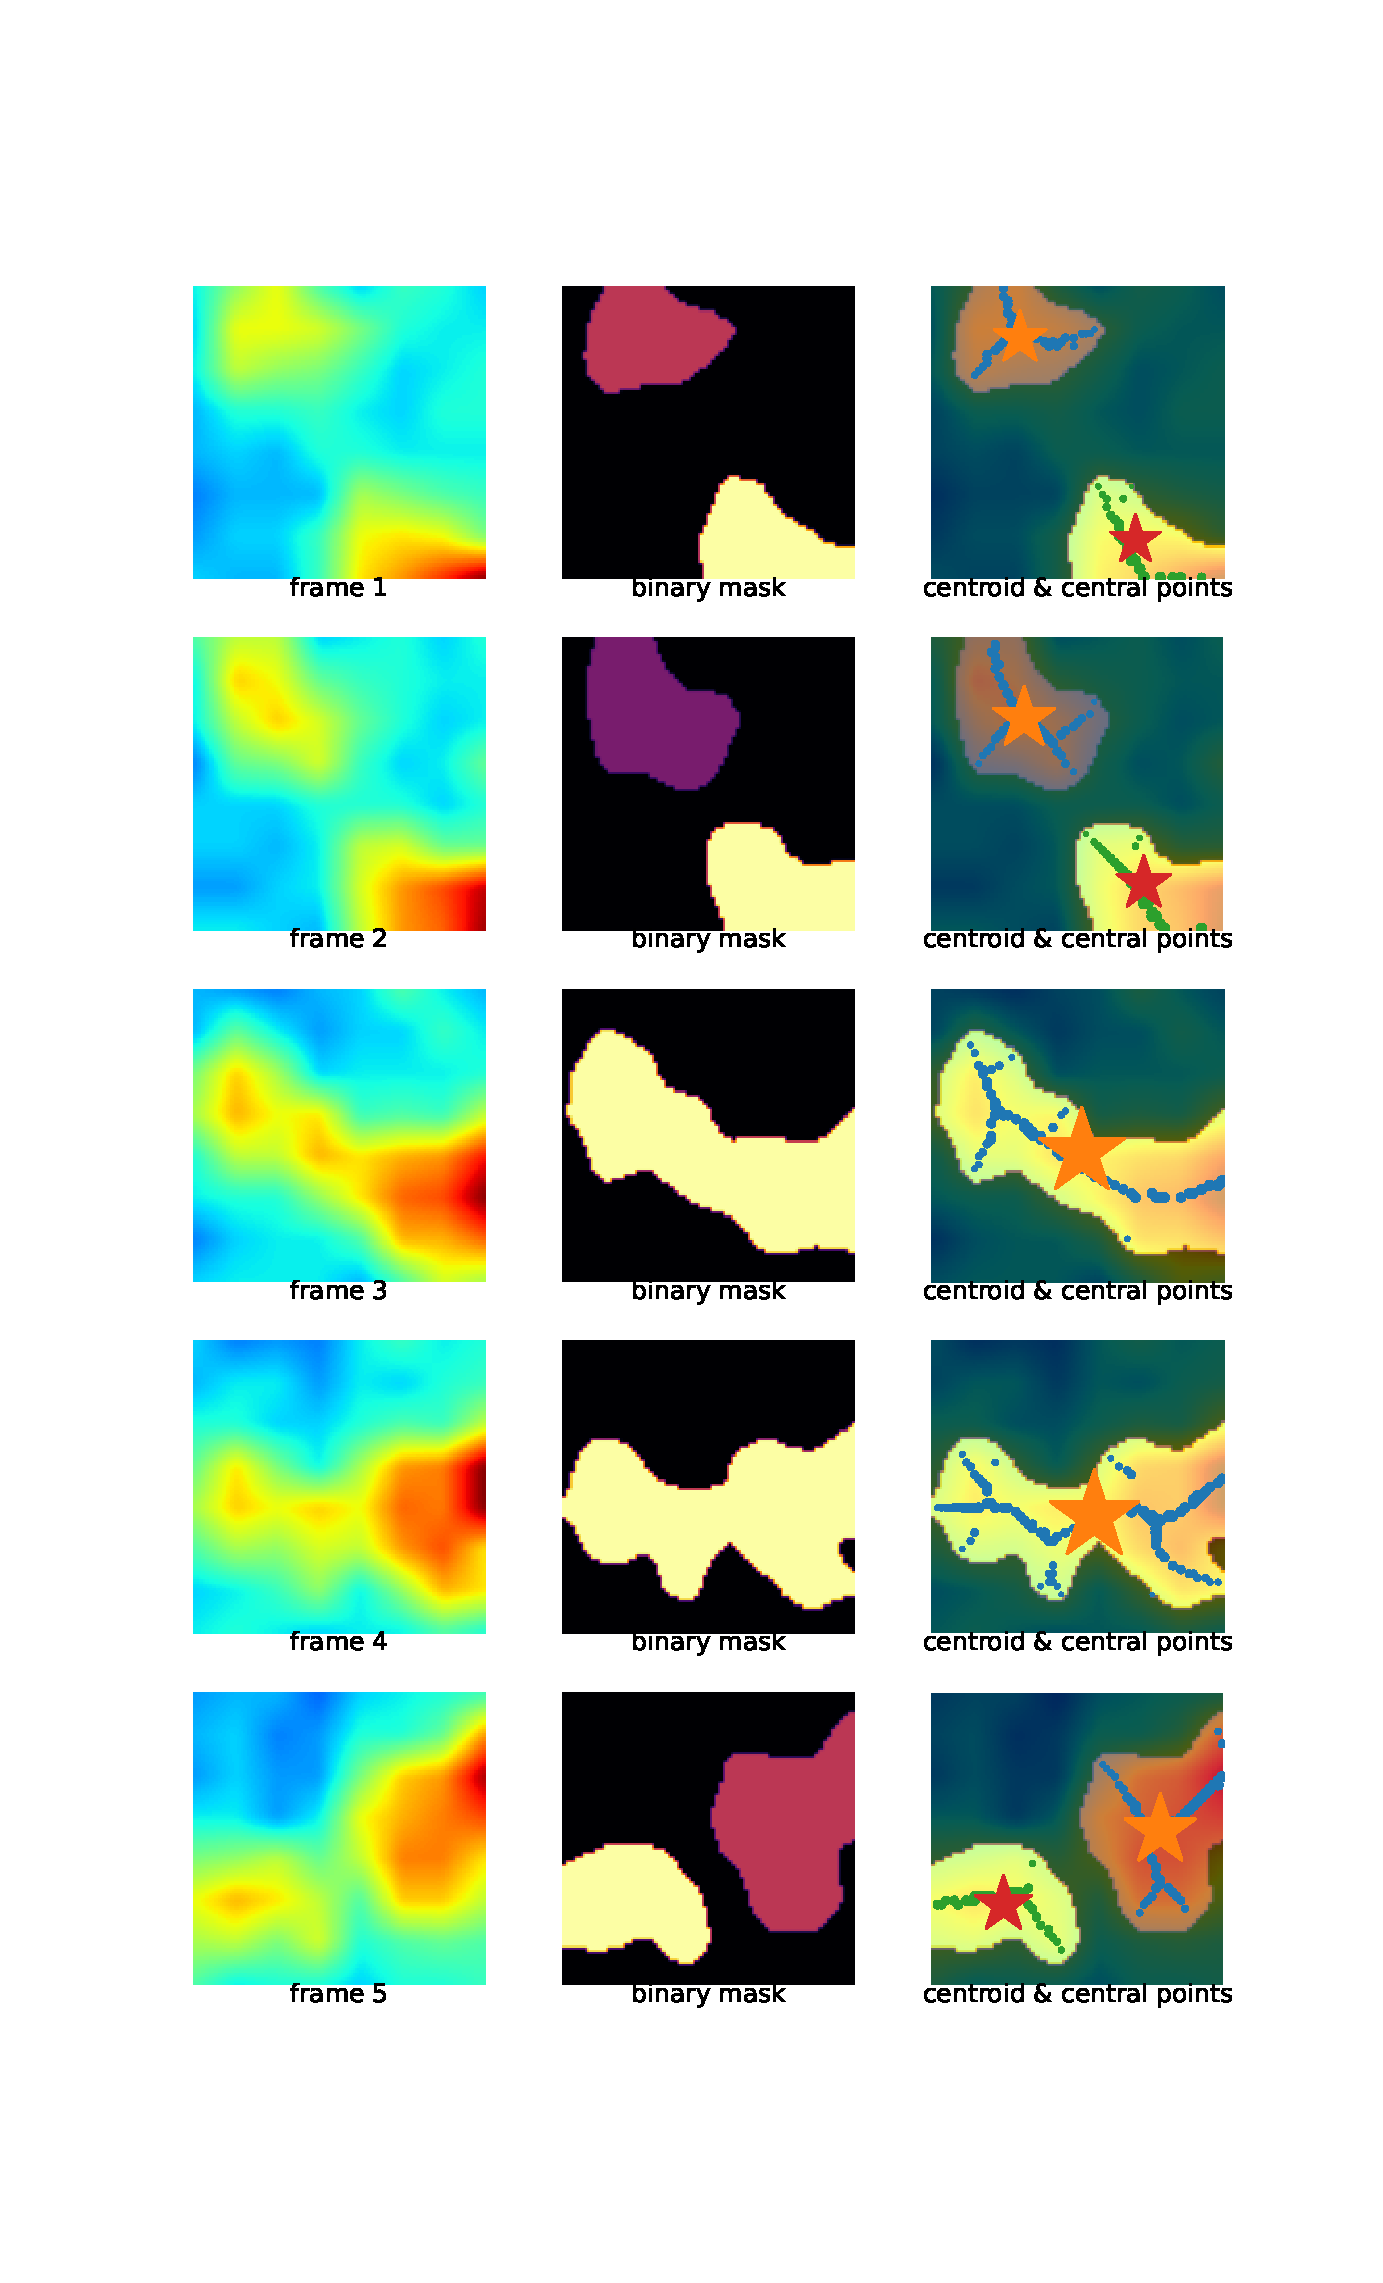
\includegraphics[width=0.6\textwidth]{figures/blobmerge.eps}
  \caption{An example frame sequence showing the blob merging issue. Left column is the interpolated image, middle column is the blob mask and right column shows the extracted feature. The star symbol represents the centroid location and the size of the star represents the size of the blob. Other round dots scattered inside the blob represent central points.}\label{fig:blobmerge}
\end{figure}

We follow the research of \cite{sharma2012blob}, adding ``central points'' as additional feature for blob representation. Central points of a blob are those points that are far away from the background, they can be found out by picking local maxima in a distance transform of the blob mask.
\subsection{Distance Transformation}
A distance transform of a binary image labels every pixel of the image by the distance between that pixel and the nearest background pixel \cite{bailey2004efficient}, which could be denoted as \autoref{eq:distancetransform}.
\begin{equation}\label{eq:distancetransform}
  I_d(x,y) = \left\{\begin{array}{cc}
               0 & I(x,y)\in\{Bg\} \\
               \min\left(\Vert x-x_0,y-y_0\Vert\right),\forall I(x_0,y_0)\in Bg & I(x,y)\in\{Ob\}
             \end{array}\right.
\end{equation}
The $\Vert\cdot\Vert$ symbol is a distance definition, could be $L_1$, $L_2$, $L_{max}$ or any other distance metric. To our concern, the distance is measured in Euclidean metric, namely $\Vert x,y\Vert=\sqrt{x^2+y^2}$.

A precise computation of the Euclidean distance transform is complex. A commonly used approximation is the chamfer distance transform \cite{butt1998optimum}. The chamfer distance transform exploits the fact that the distance between of each pixel to its nearest background pixel depends on the previously computed neighbour. The whole distance transform image could be obtained in two passes, one propagating from the upper-left corner to the lower-right corner and the other reversely. Mathematically, the two-pass algorithm with a $3\times3$ window could be written as \autoref{eq:chamferDT}, where $r,c$ denote the row and column coordinate of a pixel respectively, $x_-$ is the distance transform value after the first pass and $x_+$ is the final value after the second pass.

At the first pass, a pixel's distance to the background is propagated from three pixels above it and the one on the left of it. Two vertical and horizontal connected pixel contribute to the transform value by an distance increment of $a$, while two diagonal connected pixel contribute and increment by $b$. The value $a$ and $b$ depend on the desired approximation and usually $a\le b$. The transform result of the first pass is the minimal value among four candidates. After the first pass, those pixels at the bottom or at the lower-right corner will have the largest distance value (to the upper-right background pixel). The second pass is analogue to the first pass. Except for four neighbour pixel below and on the right, the previous result from the first pass becomes the fifth candidate. At the beginning of the second pass, the distance transform of those pixels at the bottom and lower-right corner will be iteratively replaced by values propagated from their neighbourhood because they are closer to the lower-right background pixel. After passing the object's geometry center, the results from the first pass will dominate the final result.

There are various choices for value $a$ and $b$. We use the taxicab distance $a=1$ and $b=2$. The result of distance transform is shown in \autoref{fig:DTafterfilter}.
\begin{align}\label{eq:chamferDT}
  x_-(r,c) = \min\left\{\left(\begin{array}{ccc}
                          x_-(r-1,c-1) & x_-(r-1,c) & x_-(r-1,c+1) \\
                          x_-(r,c-1)\\
                        \end{array}  \right)+
                        \begin{pmatrix}
                          b & a & b \\
                          a & - & - \\
                          - & - & -
                        \end{pmatrix} \right\}
\\
  x_+(r,c) = \min\left\{
            \left(\begin{array}{ccc}
                         &x_-(r,c)&x_+(r,c+1)\\
            x_+(r+1,c-1)& x_+(r+1,c) &x_+(r+1,c+1)
                        \end{array}
                        \right)+
                        \begin{pmatrix}
                          - & - & - \\
                          - & 0 & a \\
                          b & a & b
                        \end{pmatrix}
                        \right\}
\end{align}
\subsection{Local Maxima in a Distance Transform}
By the definition of distance transform, a distance transform of a binary blob mask is essentially a local shape descriptor. The distance value of a pixel only depends on the size of its \emph{local convex region}. Another concatenated blob has little influence to the distance transform result except the overlapped pixels.

However, not all of the distance values are equally interesting. Ideally, only two points representing the location of the merged blobs are needed to track two merged blobs. One way to find local region centers is to filter the distance values by whether they are close to the maximum distance value in the distance transform. The fourth column in \autoref{fig:DTafterfilter} shows the result. This method assumes that the size of two merged blobs are similar, otherwise most of the detected points will be located within the larger object or the small object is eventually not detected at all. The advantage of this method is that all the detected points do locate in the blob center.

\citeauthor{sharma2012blob} \cite{sharma2012blob} determines the central points by applying a $3\times3$ filter to extract all the local maxima, and filtering out the local maxima that are smaller than $50\%$ of the maximum distance value. However, their work focus on side-view RGB images and cannot be directly transferred to our use case.

We extract the local maxima by an edge detector inspired by the Laplacian filter. A Laplacian filter is commonly used in grayscale images to find out the points where pixel intensity changes fiercely. In the discrete world, a Laplacian filter could be a $3\times3$ convolution kernel written as the following \autoref{eq:laplacian}. Intuitively speaking, a Laplacian filter compares the intensity of a pixel with its four neighbours, multiplying the intensity of the center pixel by 4 and subtracting the intensity of surrounding pixels. In a homogenous region when all five pixels have the same intensity, the computation result would be zero. At the border of a image, half of the kernel locate inside the object, having a brighter pixel, and half of the kernel fall into the background (darker therefore the pixel value is lower). The result of \autoref{eq:laplacian} would be greater than zero and that pixel would be marked as a boarder pixel.
\begin{equation}\label{eq:laplacian}
  \begin{pmatrix}
    0 & -1 & 0 \\
    -1 & 4 & -1 \\
    0 & -1 & 0
  \end{pmatrix}
\end{equation}

Similarly, the second column in \autoref{fig:DTafterfilter} shows that the local maxima of our top-view images looks like a ``border'' that separates the entire blob into two symmetric parts. Based on the idea of a edge detector, we propose the filter shown in \autoref{eq:filterkernel} and the results are shown in the third column of \autoref{fig:DTafterfilter}.
\begin{equation}\label{eq:filterkernel}
  \begin{pmatrix}
    -1 & -2 & -1 \\
    -2 & 12 & -2 \\
    -1 & -2 & -1
  \end{pmatrix}
\end{equation}

This method ensures that every convex part of the blob obtains a point representation, so it will not miss out any part of a blob. However, many redundant points are also included in the final blob representation, which may cause a match failure in the tracking stage. Imagine the following common scenario: when a blob moves at a constant speed and several frames are captured. In the second frame, comparing with the true geometry center, the local maxima points near the blob edge will always be closer to the blob's previous location. Therefore the matched object location is lagging behind its actual position. Then in the third frame, the matching is made between a previous border point and a current border point. If the human moves a little bit faster, the distance between the previous border point and any current point would exceed the nearest neighbour threshold. A matching is lost.

Considering the robust point representation it can offer, we still choose this method for feature extraction, and solve the possible matching failure in the tracking layer.
\begin{figure}
  \centering
  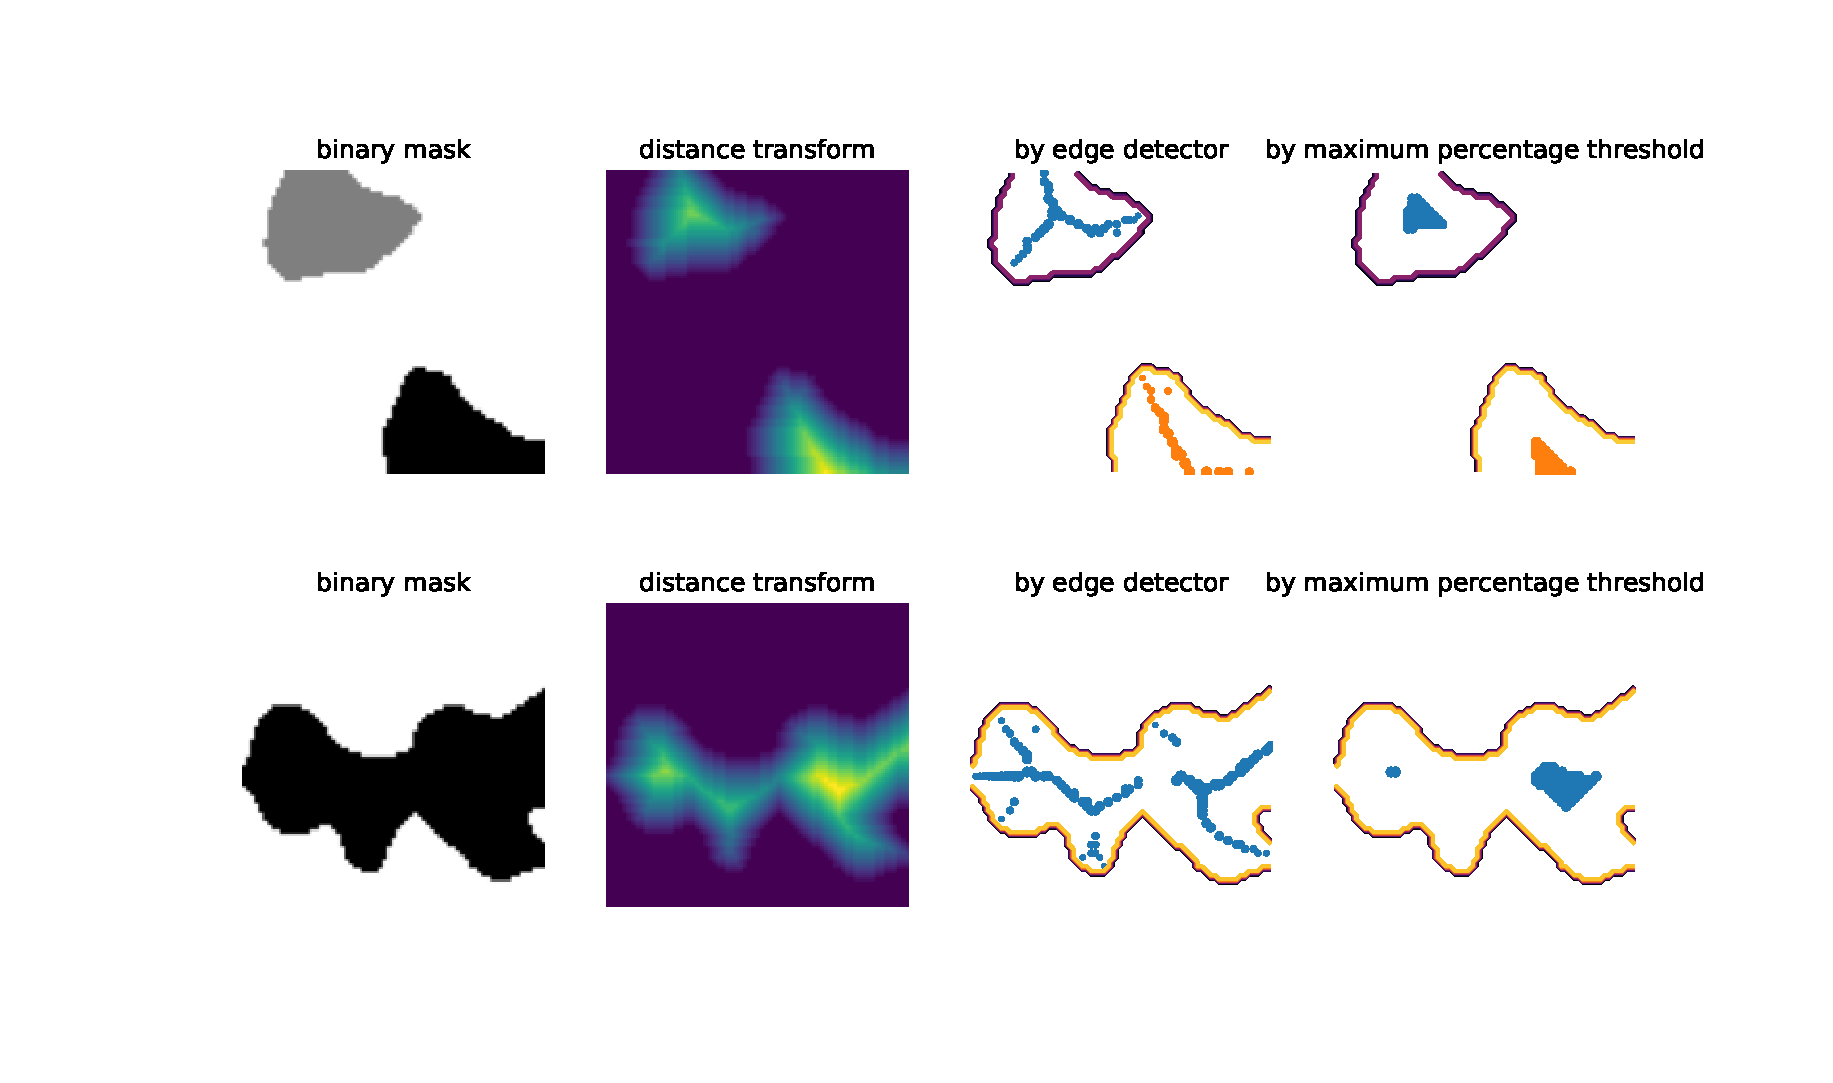
\includegraphics[width=\textwidth]{figures/centralsbyfilter.eps}
  \caption{The first two columns show the original mask and its distance transform result. In the second column, a brighter pixel indicates a higher distance to the background. The third column shows the central points extracted by a edge detector. The fourth column shows central points found by a percentage filter ($> 80\%$) of the highest distance value.}
  \label{fig:DTafterfilter}
\end{figure}

\subsection{Informativity and Stability of Central Points}
Central points preserve most information about the original blob. If the distance value to the background of every central point is preserved, the original blob mask could be approximately recovered from the central points, see \autoref{fig:maskrecover}. In contrary, the shape information is lost when using the centroid representation. Certainly, multiple central points require more memory space than a single centroid, but the central points representation compresses information efficiently. Based on our observation, the ratio of cental points and blob size is around $4\%\sim6\%$: a blob with size 1200 has around 70 central points and a blob with size 500 has around 30 pixels. Therefore, we have reduced the memory usage for every blob by $95\%$ while still kept most information.
\begin{figure}
  \centering
  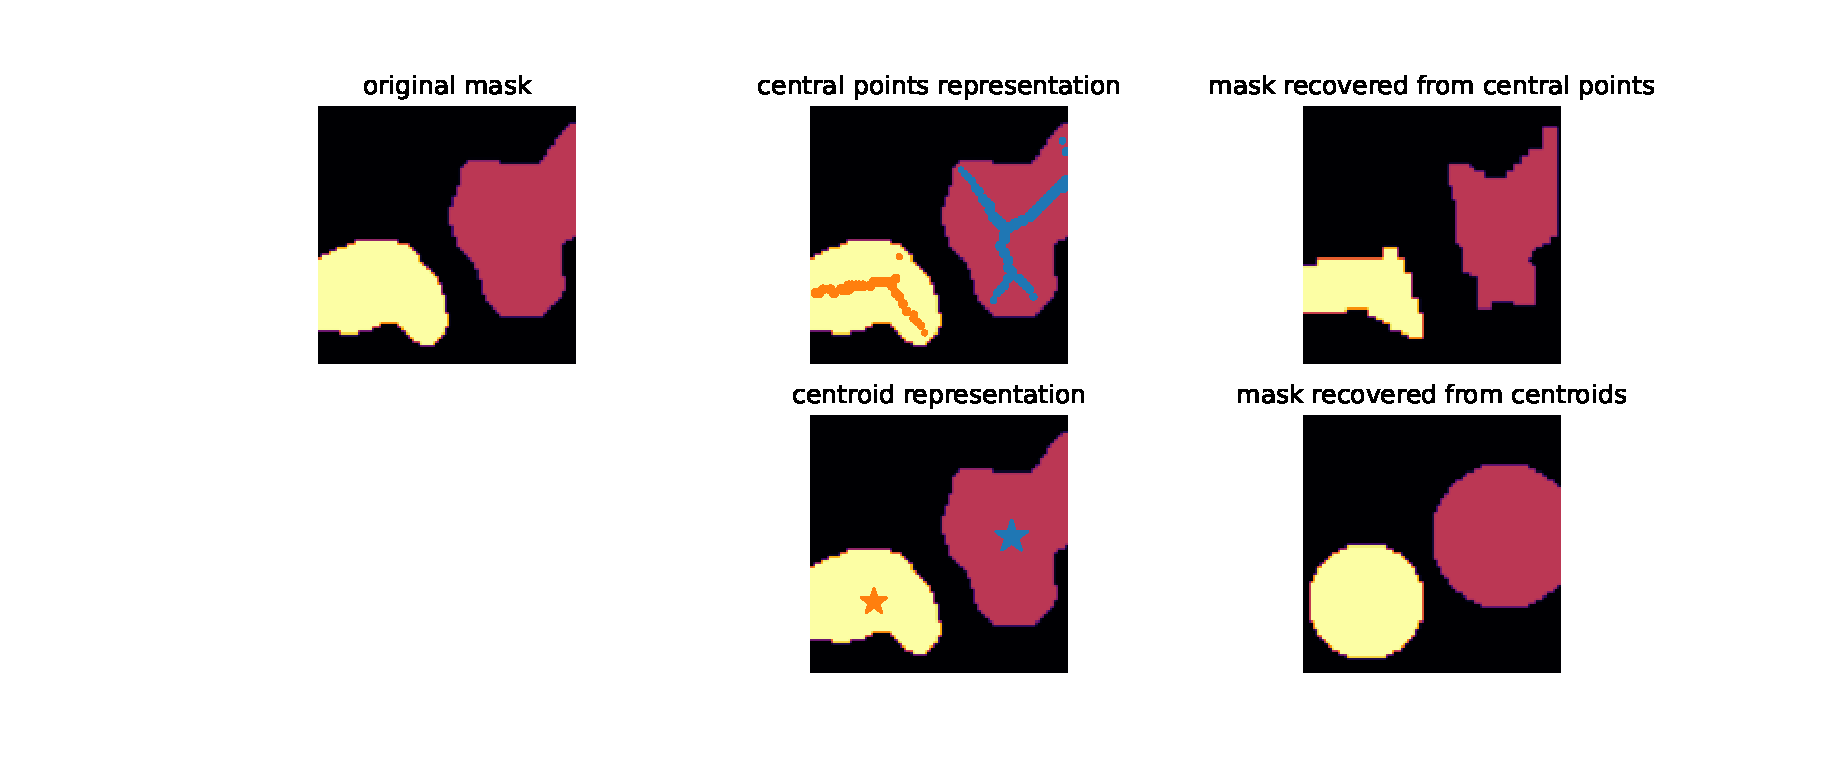
\includegraphics[width=\textwidth]{figures/maskrecover.eps}
  \caption{Mask recovery from the central points shows most of the shape information is preserved}\label{fig:maskrecover}
\end{figure}

The above analysis shows that the central point representation is a stand-alone feature describer, and is independent of the centroid representation. However, because we cannot reduce the number of central points to a low level, the tracking algorithm must find the optimum candidate among all central points, which brings about extra computational cost that is wasted when blobs are not merged. Therefore, we describe the blobs by two representations (see \autoref{eq:blobdenote2}, $P$ is the coordinate of a central point and $D$ is its distance to the background). And would only switch to central points matching if the centroid matching fails. Details about matching are elaborated in \Cref{sec:track}.
\begin{equation}\label{eq:blobdenote2}
  \begin{split}
        B = &\{C,S\}; \\
        &\{(P_1,D_1),(P_2,D_2),\cdots,(P_n,D_n)\}
      \end{split}
\end{equation}

The cluster of central points looks like the ``spine'' of the original blob. This is not surprising because we visually examine the shape of the local maxima points in \autoref{fig:DTafterfilter}. Actually, the set of local maxima points in a distance transform are an approximation to the medial axis of a binary mask \cite{lee1996chessboard}, see \autoref{fig:medialaxisandcentral}. A medial axis of a $R^2$ shape is the set of points that have more than one closest point on the object's contour line. \citeauthor{attali2009stability} \cite{attali2009stability} proved that for shapes in $R^2$, fluctuation of the shape contour only effect part of the branches of the medial axis. This partially explains why the central points stay stable by blob merging/ splitting.
\begin{figure}
  \centering
  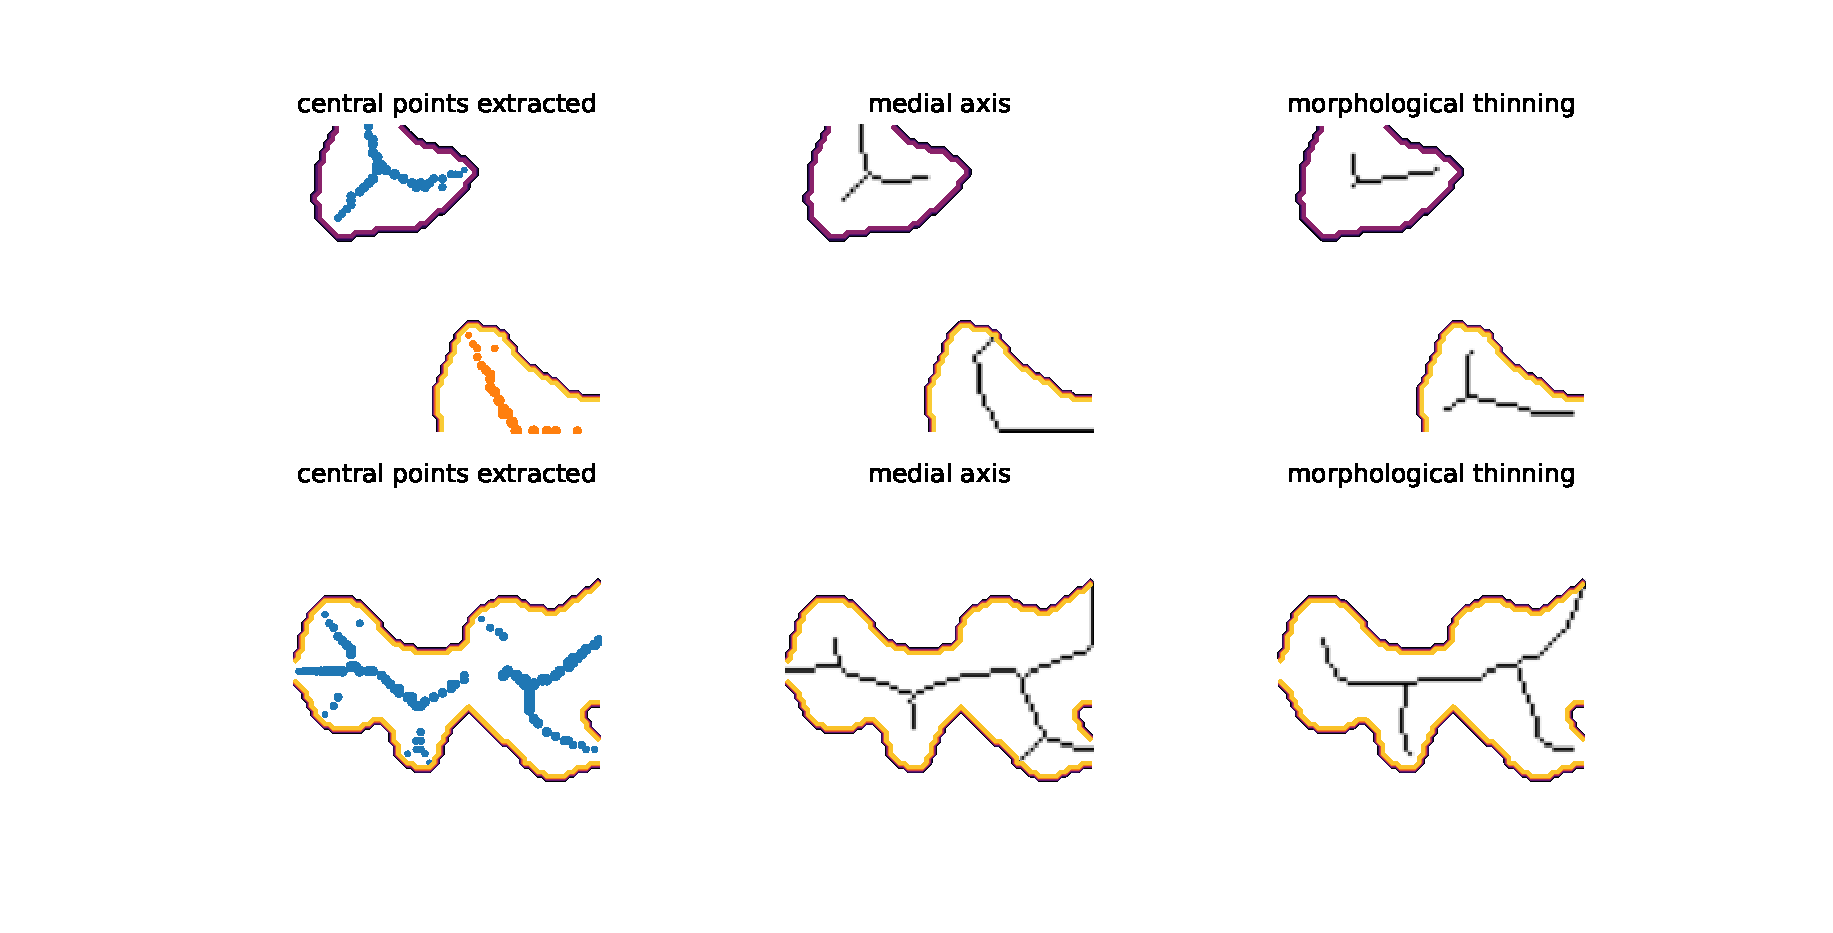
\includegraphics[width=\textwidth]{figures/centralandmedial.eps}
  \caption{The first column shows the set of central points, the second column is the medial axis of the same binary mask. The third column shows result of another thinning algorithm by \cite{zhang1984fast}.}\label{fig:medialaxisandcentral}
\end{figure}




\section{Human Object Tracking} \label{sec:track}
\chapter{Performance Evaluation} \label{ch:evaluation}
\section{Evaluation in Controlled Environment}
The counting device was firstly mounted at a household doorframe to test its accuracy. The mounting height was about 2 meters and the ambient temperature was around $24^\circ C$. In a 40 minutes test, a test person was asked to enter and exit the room continuously for 100 times. The user interface shown in \autoref{fig:noderedui} was turned on in a smartphone so that the test person can read the algorithm output immediately.

The algorithm detects 94 enter events correctly and 97 exit events correctly. And it has successfully handled multiple-human events, such as sequential entering and passing in opposite directions.
\section{Evaluation in Uncontrolled Environment}
The counting device has also been attached to the ceiling of the main entrance in our faculty department to evaluate its performance in real situations. The mounting height was a little higher than the previous experiment, at about 3 meters. The device has operated for two weeks around the clock, except for the first 2 days in the second week because of a local network update. The device transmits the counting result of the proposed algorithm as well as the actual infrared image for later annotation. By this way, we have collected a valid dataset of 8 days in total. The evaluation time slot begins from 8:00 in the morning and ends at 20:00.

The ground truth is annotated by manually iterating through all received images. For ease of examination, the device has only transmitted images when there are three pixels hotter than ambient temperature. Usually, the image transmission begins when a human enters the camera FOV and terminates when the human leaves. We regard each video sequence as one individual event (or two closely happening events). A timestamp was attached to each video sequence to indicate the time of that event. By this way, the number of images to be reviewed is reduced from several hundreds of thousands to a moderate number of around one thousand.

The manual ground truth annotation can only locate the time of event occurrence to minutes. However, the counting algorithm outputs an accurate millisecond timestamp when the count changes. This time disparity in timestamp has caused difficulty in matching the ground truth and the algorithm output with automatic tools. Therefore the accuracy evaluation is carried out visually. For every ground truth enter or exit event, it is checked if the counting algorithm outputs a correct result (+1 for entering and -1 for exiting) in the nearby 30 seconds. If this is the case we add one to the correct counting category otherwise to the wrong counting category. A false detection, when no event is observed in the ground truth video sequence but the algorithm outputs a non-zero value, also falls into the wrong counting category. See \autoref{fig:ESKibana} for example, the event around 12:00 is a false detection and the event around 14:00 is a wrong counting, both will increase the number of ``wrong counting'' by one.

We have also picked out those events which involve multiple humans entering or exiting simultaneously and evaluated them separately. For such events, correct counting consists of the correct movement direction as well as the correct counting number. The counting of a multiple-human event is only regarded correct when the algorithm outputs the exact human number as observed in the ground truth. Take \autoref{fig:ESKibana} as an example, the long green bar plots around 11:20 and 16:00 are two correctly counted multiple-human events, and the events around 13:00 and 14:00 are wrong counting. Note that sometimes the algorithm outputs ``+2'' and two single entering events are observed at that time point, we regard such events as correctly counted.

The dataset statics are shown in \autoref{tab:eva_data}, all data are grouped in 2-hour time ranges. We have finally counted 222 correct and 50 wrong outputs in single human events, which amounts to an accuracy of 81.6\%. There have also been 10 correct and 6 wrong outputs in multiple-human events, which amounts to an accuracy of 62.5\%. The overall accuracy is around 80\%.

\begin{table}[]
\small
\begin{tabular}{l|ll|ll|l|ll|ll|}
\cline{2-5} \cline{7-10}
                            & \multicolumn{2}{l|}{single-human event} & \multicolumn{2}{l|}{multi-humans event} &       & \multicolumn{2}{l|}{single-human event} & \multicolumn{2}{l|}{multi-humans event} \\ \hline
\multicolumn{1}{|l|}{Day1}  & correct             & wrong             & correct             & wrong             & Day2  & correct             & wrong             & correct             & wrong             \\ \hline
\multicolumn{1}{|l|}{8:00}  & -                   & -                 & -                   & -                 & 8:00  & 5                   & 1                 & -                   & -                 \\
\multicolumn{1}{|l|}{10:00} & -                   & -                 & -                   & -                 & 10:00 & 10                  & 4                 & 1                   & 0                 \\
\multicolumn{1}{|l|}{12:00} & 9                   & 1                 & -                   & -                 & 12:00 & 11                  & 1                 & 0                   & 2                 \\
\multicolumn{1}{|l|}{14:00} & 4                   & 0                 & 1                   & 0                 & 14:00 & 24                  & 5                 & 1                   & 1                 \\
\multicolumn{1}{|l|}{16:00} & 5                   & 0                 & 0                   & 1                 & 16:00 & 9                   & -                 & -                   & -                 \\
\multicolumn{1}{|l|}{18:00} & 5                   & 1                 & -                   & -                 & 18:00 & -                   & -                 & -                   & -                 \\ \hline
\multicolumn{1}{|l|}{Day3}  & correct             & wrong             & correct             & wrong             & Day4  & correct             & wrong             & correct             & wrong             \\ \hline
\multicolumn{1}{|l|}{8:00}  & 8                   & 2                 & -                   & -                 & 8:00  & -                   & -                 & -                   & -                 \\
\multicolumn{1}{|l|}{10:00} & 5                   & 1                 & -                   & -                 & 10:00 & -                   & 1                 & -                   & -                 \\
\multicolumn{1}{|l|}{12:00} & 0                   & 1                 & 0                   & 1                 & 12:00 & 1                   & 1                 & -                   & -                 \\
\multicolumn{1}{|l|}{14:00} & 2                   & 0                 & 2                   & 0                 & 14:00 & 5                   & 2                 & -                   & -                 \\
\multicolumn{1}{|l|}{16:00} & 2                   & 0                 & -                   & -                 & 16:00 & 2                   & 1                 & 3                   & 0                 \\
\multicolumn{1}{|l|}{18:00} & -                   & -                 & -                   & -                 & 18:00 & -                   & -                 & -                   & -                 \\ \hline
\multicolumn{1}{|l|}{Day5}  & correct             & wrong             & correct             & wrong             & Day6  & correct             & wrong             & correct             & wrong             \\ \hline
\multicolumn{1}{|l|}{8:00}  & -                   & -                 & -                   & -                 & 8:00  & 7                   & 1                 & -                   & -                 \\
\multicolumn{1}{|l|}{10:00} & 0                   & 3                 & 0                   & 1                 & 10:00 & 1                   & 0                 & -                   & -                 \\
\multicolumn{1}{|l|}{12:00} & 7                   & 4                 & -                   & -                 & 12:00 & 6                   & 1                 & -                   & -                 \\
\multicolumn{1}{|l|}{14:00} & 7                   & 0                 & 1                   & 0                 & 14:00 & 8                   & 1                 & -                   & -                 \\
\multicolumn{1}{|l|}{16:00} & -                   & -                 & -                   & -                 & 16:00 & 4                   & 0                 & -                   & -                 \\
\multicolumn{1}{|l|}{18:00} & -                   & -                 & -                   & -                 & 18:00 & 3                   & 1                 & -                   & -                 \\ \hline
\multicolumn{1}{|l|}{Day7}  & correct             & wrong             & correct             & wrong             & Day8  & correct             & wrong             & correct             & wrong             \\ \hline
\multicolumn{1}{|l|}{8:00}  & -                   & -                 & -                   & -                 & 8:00  & 2                   & 0                 & -                   & -                 \\
\multicolumn{1}{|l|}{10:00} & 1                   & 3                 & -                   & -                 & 10:00 & 2                   & 0                 & -                   & -                 \\
\multicolumn{1}{|l|}{12:00} & 9                   & 1                 & -                   & -                 & 12:00 & 5                   & 1                 & -                   & -                 \\
\multicolumn{1}{|l|}{14:00} & 9                   & 2                 & 1                   & 0                 & 14:00 & 13                  & 3                 & -                   & -                 \\
\multicolumn{1}{|l|}{16:00} & 8                   & 3                 & -                   & -                 & 16:00 & 18                  & 3                 & -                   & -                 \\
\multicolumn{1}{|l|}{18:00} & 4                   & 1                 & -                   & -                 & 18:00 & 1                   & 0                 & -                   & -                 \\ \hline
\end{tabular}
\caption{Dataset statistics. The "-" symbol means entry is not applicable.}\label{tab:eva_data}
\end{table}

\section{Discussion}
To investigate what has caused the performance drop in the real situation, the observed possible issues have been categorized into five classes. And they are:
\begin{enumerate}
  \item Not detected: when a hot object is observed in the ground truth but the algorithm does not respond at all.
  \item Noise: when there is only random temperature fluctuation in the scene but the algorithm reports an object entering or leaving.
  \item Long sequence: when a human stands beneath the camera for a long period (several minutes).
  \item Heat disturbance: when the background temperature is not homogenous in the whole scene, for example, half of the FOV monitoring the sunny side of a doorway has a higher temperature.
  \item Missing frame: when somehow a few frames in a video sequence is not captured, which causes an abrupt position change of the detected object.
\end{enumerate}
\autoref{fig:eva_errors} shows the occurrence frequency of the aforementioned issues. Among which the ``missing frame'' error turned out to be the most common but also the most devastating issue that drastically reduced the accuracy of the proposed algorithm.
\begin{figure}
  \centering
  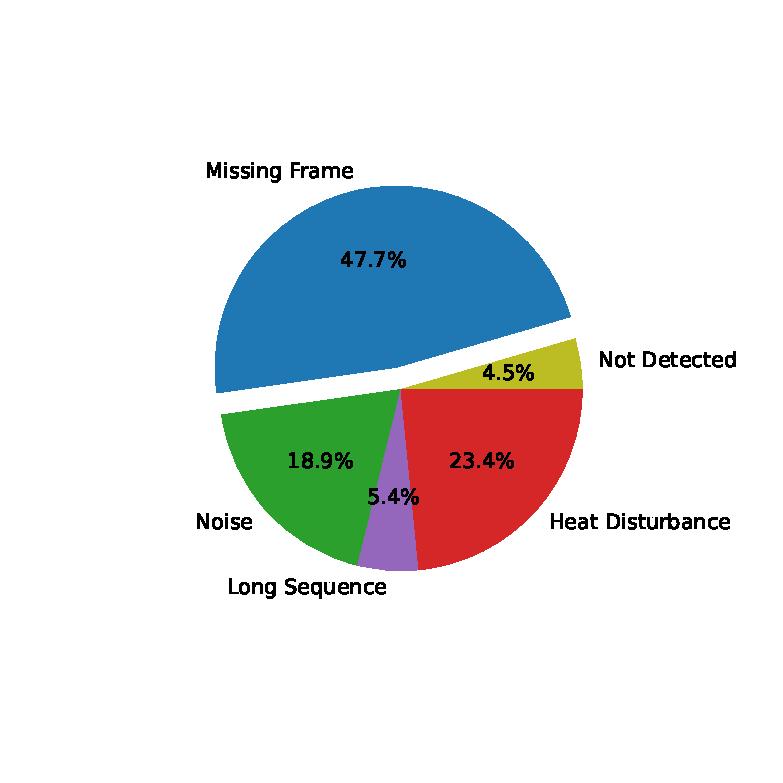
\includegraphics[width=0.6\textwidth]{figures/errors.eps}
  \caption{The percentage distribution of issues that may cause a detection or tracking failure.}\label{fig:eva_errors}
\end{figure}

\subsection{Missing Frame Error}
\begin{figure}
  \centering
  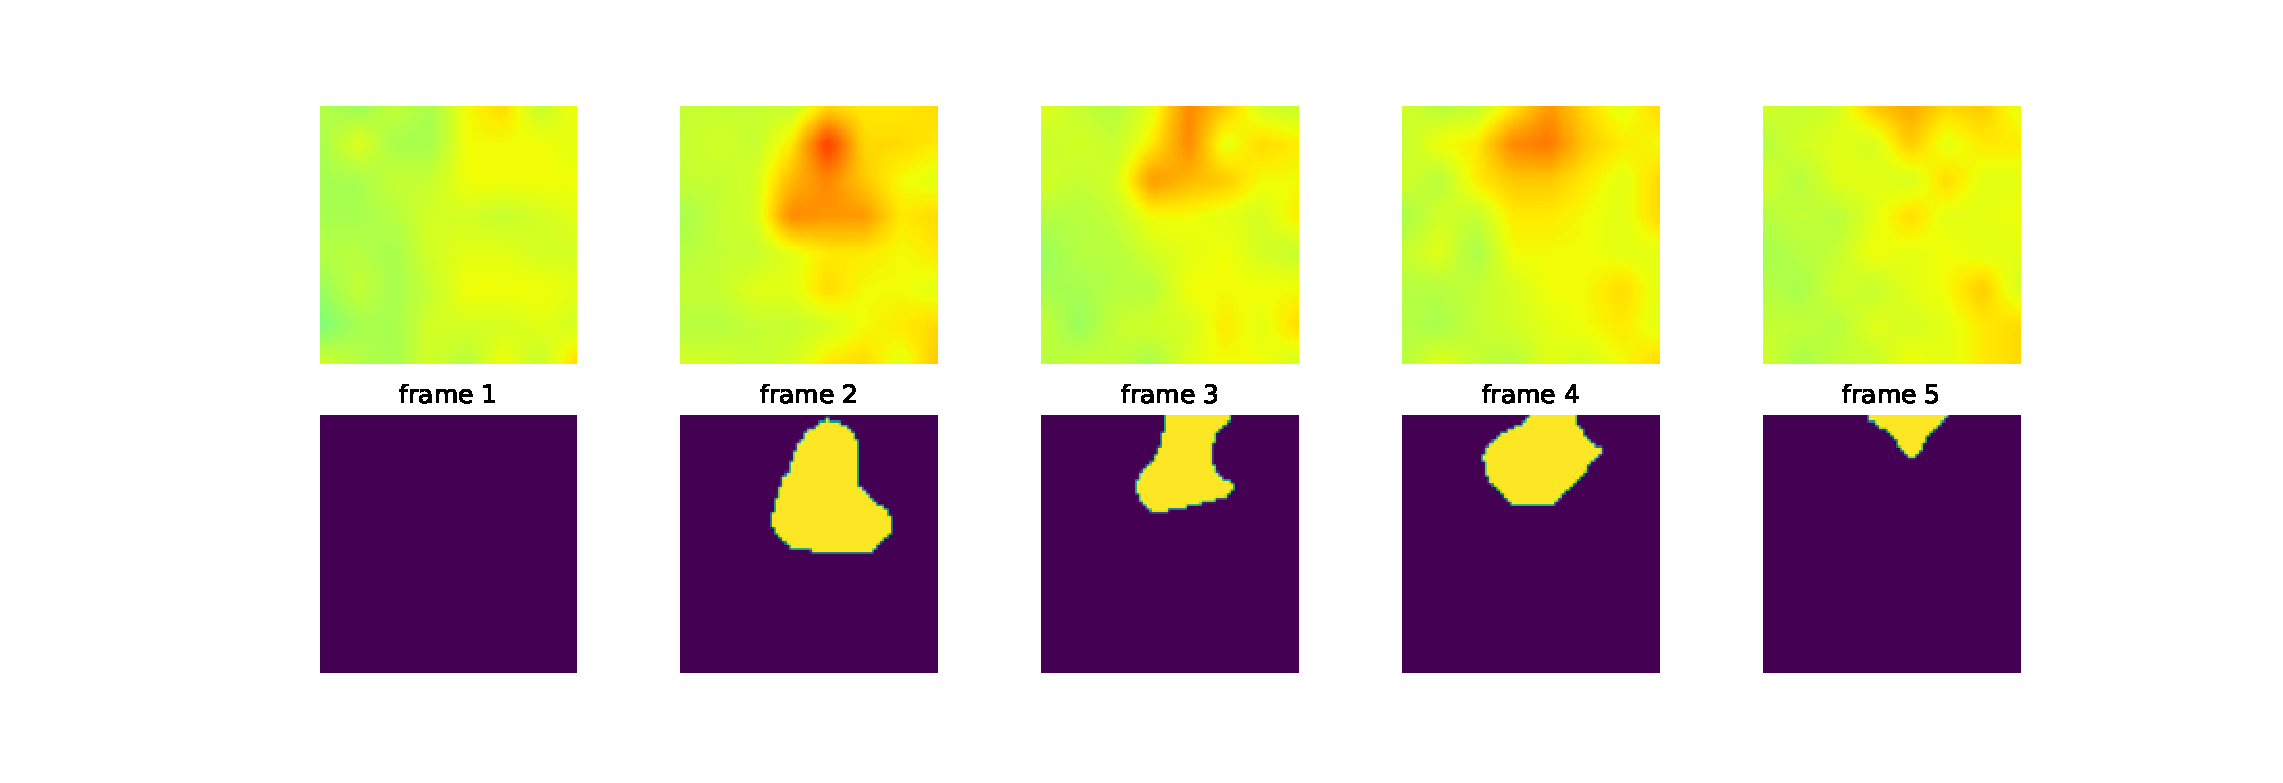
\includegraphics[width=\textwidth]{figures/err_missingframe.eps}
  \caption{This example shows an exit event where only the last few frames are captured, the missing frames of the event beginning makes it impossible to track and count the event correctly. The first row is the IR camera readings and the second row is the object mask.}\label{fig:err_mf}
\end{figure}
\autoref{fig:err_mf} demonstrates a typical detection failure that several beginning frames of an event are missed out. A further investigation shows this issue may be traced back to a network lagging. As mentioned in \Cref{ch:platform}, all the messages from the microcontroller are transmitted through a public MQTT broker so that realtime feedback can be obtained by running a listener client elsewhere. As contrary, in the controlled environment, both message publisher and listener locate under the same network and a local MQTT broker is used. Sending the messages to the Internet must have taken more time. Most of the message content is the raw IR image, which takes around 320 bytes. At a frame rate of 10 fps (when a human is detected), the generated data flow is about 3.5KB per second. Though the amount of data is still quite trivial, it is already larger than a common IoT application. Considering we use a public broker and the broker provider may have restrictions in the data amount, the network connection may deteriorate and finally cause a pause in the processing loop.

Moreover, the structure of the program could be improved. In the initial design, the message sending function is called within the tracking algorithm. Because it is observed that sending an image takes no longer than several milliseconds and will not break the time restriction for realtime processing. However, providing that a message sending may take several tens of milliseconds, the publishing task should be offloaded from the tracking algorithm. The task could be handled by another thread or even by the other CPU core. \autoref{fig:err_processloop} shows the improved program structure.
\begin{figure}
  \centering
    \subfloat[\centering the initial process loop]{{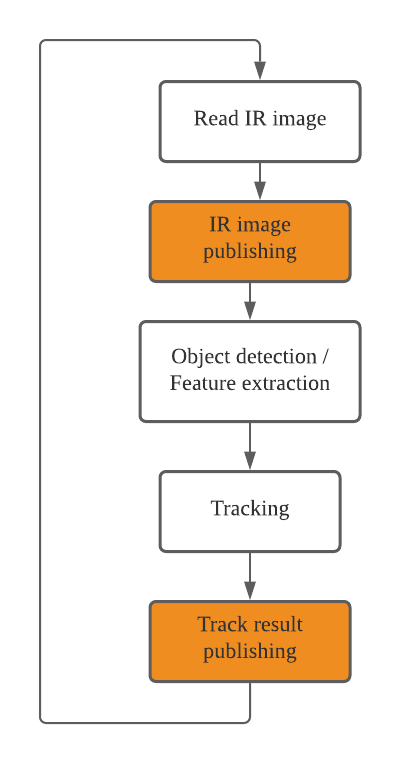
\includegraphics[width=0.3\textwidth]{figures/processloop1.png}}}%
    \qquad
    \subfloat[\centering the improved process loop]{{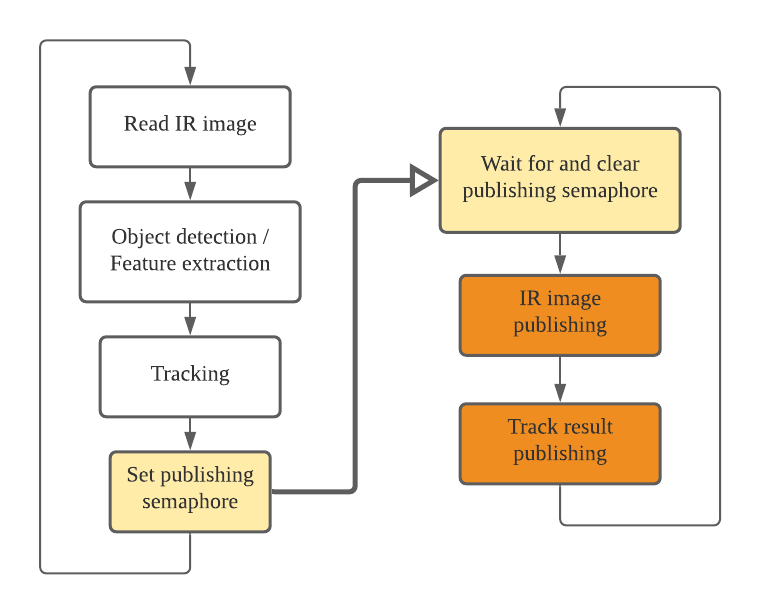
\includegraphics[width=0.6\textwidth]{figures/processloop2.png}}}%
    \caption{Initial and improved program flow. The orange blocks denote the time-consuming publishing tasks.}%
    \label{fig:err_processloop}
\end{figure}

After switching to a more stable broker, the number of missing frame error has reduced by 40\% (from 33 to 20). A lower error rate is expected when the publishing task is excluded from the process loop. Switching to a local broker instead of a public broker may also improve the network connection. Eventually, the image publishing task can be canceled totally because it is not needed in the deployment.

\subsection{Heat Disturbance Error}
\begin{figure}
  \centering
  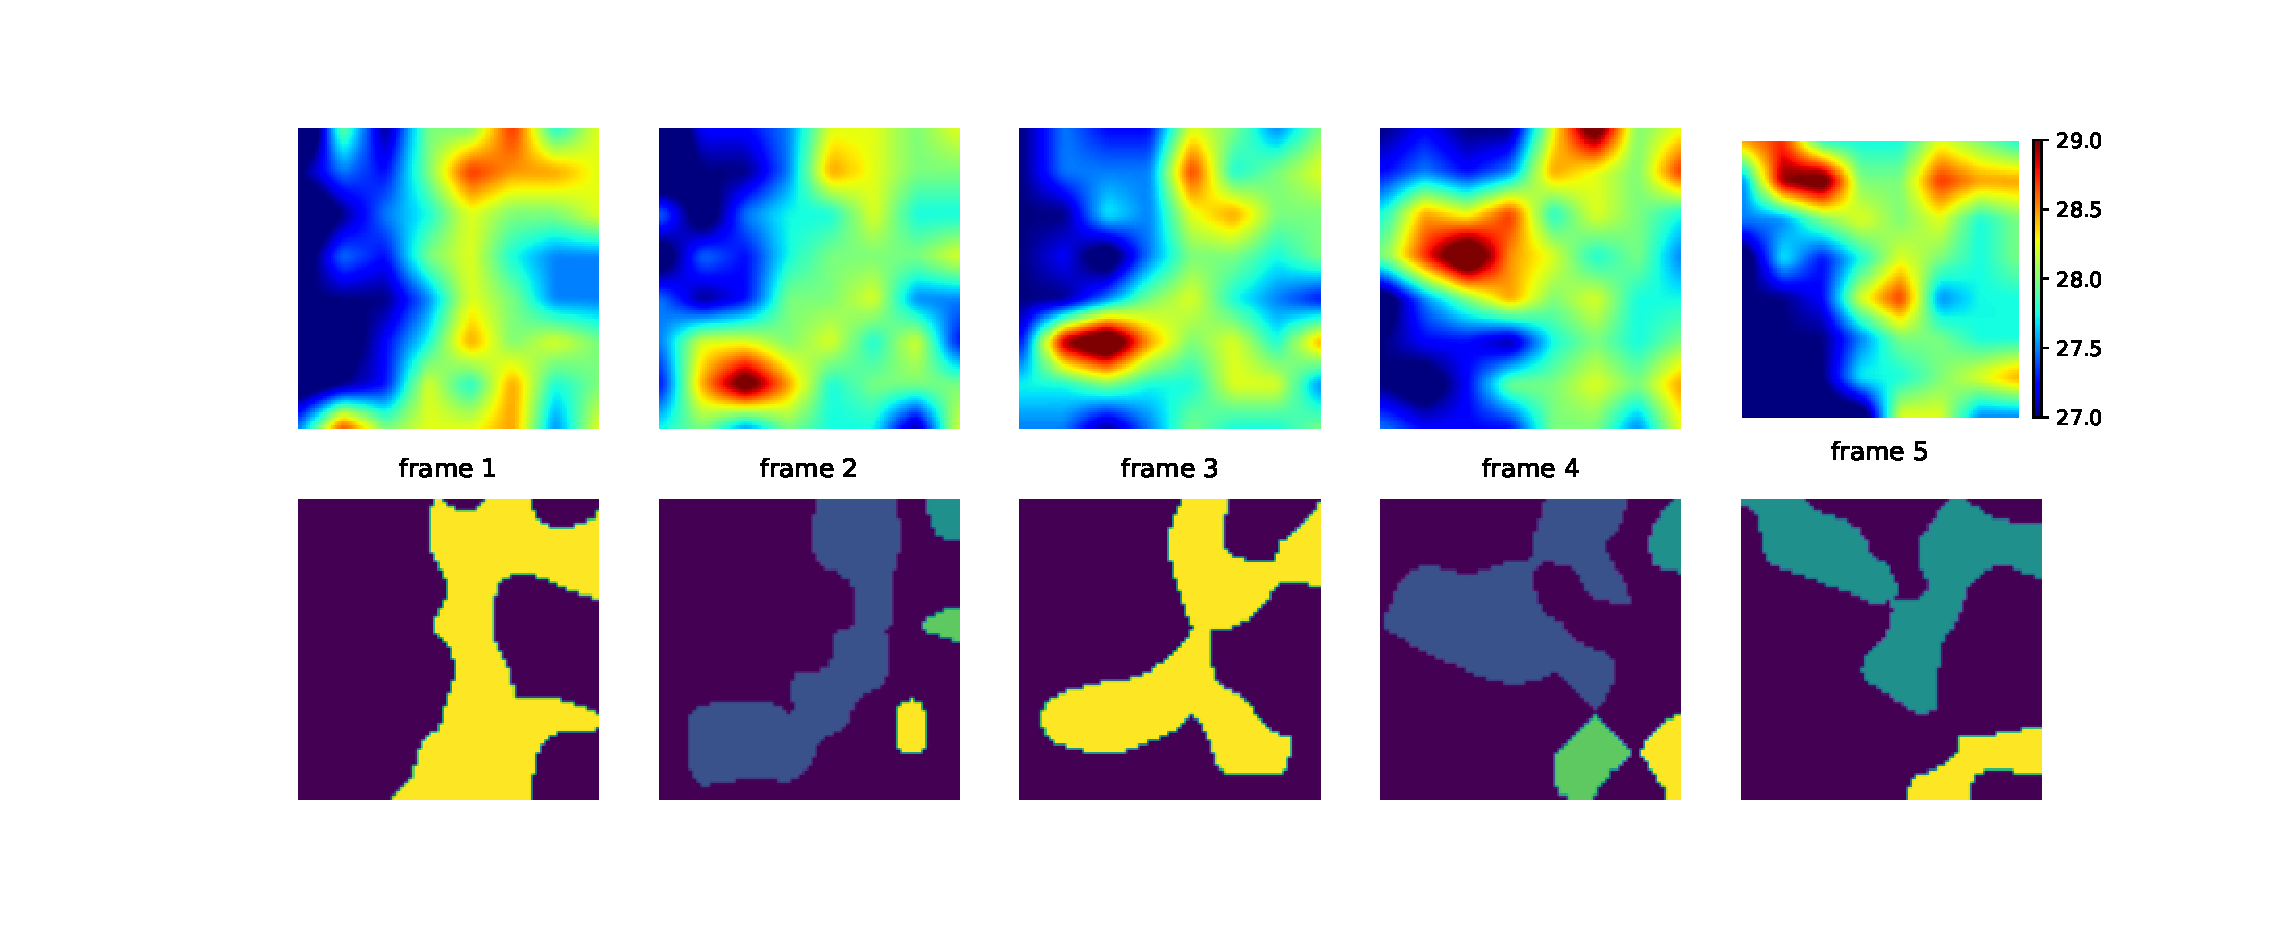
\includegraphics[width=\textwidth]{figures/err_heatdisturb.eps}
  \caption{This example shows a human leaving the room (on the left side), while half of the monitored area (on the right side) is heated up close to human body temperature. The first row is the IR camera readings and the second row is the erroneous object mask. The colorbar unit is $^\circ C$.}\label{fig:err_hd}
\end{figure}
Another frequent occurred abnormal scenario is the ``heat disturbance'' issue, where a constant heat source in the camera view interferes with the object detection procedure severely. A temperature rising in the partial background can be caused by a long time of exposure to the sunshine. A typical scenario is when only part of the floor is shined. For example, a doorway facing the direction of sunrise usually has its outer side shined and the inner side in the shadow. Several hours of sunshine is sufficient to cause a distinct temperature difference on different sides of the doorway. The developed algorithm holds the assumption that the background temperature is average within the whole camera view, and the background temperature is lower than the human body temperature. When this assumption does not hold anymore, human objects can no longer be segmented from the background. \autoref{fig:err_hd} shows that heat reflection from the ambient environment (floors, walls, etc.) can reach up to the human body temperature.

Moreover, the increased installation height has also contributed to the issue. Since the infrared ray emissivity attenuates by squared distance, the captured human body temperature becomes lower when the distance between the camera and the human increases (from 2 meters to 3 meters).

Overall, the heated ambient environment and a lower detected body temperature lead to a challenge in human object segmentation. And this segmentation challenge can not be solved by picking a well-selected threshold because the IR camera we used has an accuracy of $\pm 2.5^\circ C$. Therefore, we consider the heat disturbance issue as a hardware limit problem. A more precise segmentation should be achieved by switching to a better IR camera with higher precision.

\subsection{Other Errors and Anomalies}
\begin{figure}
  \centering
  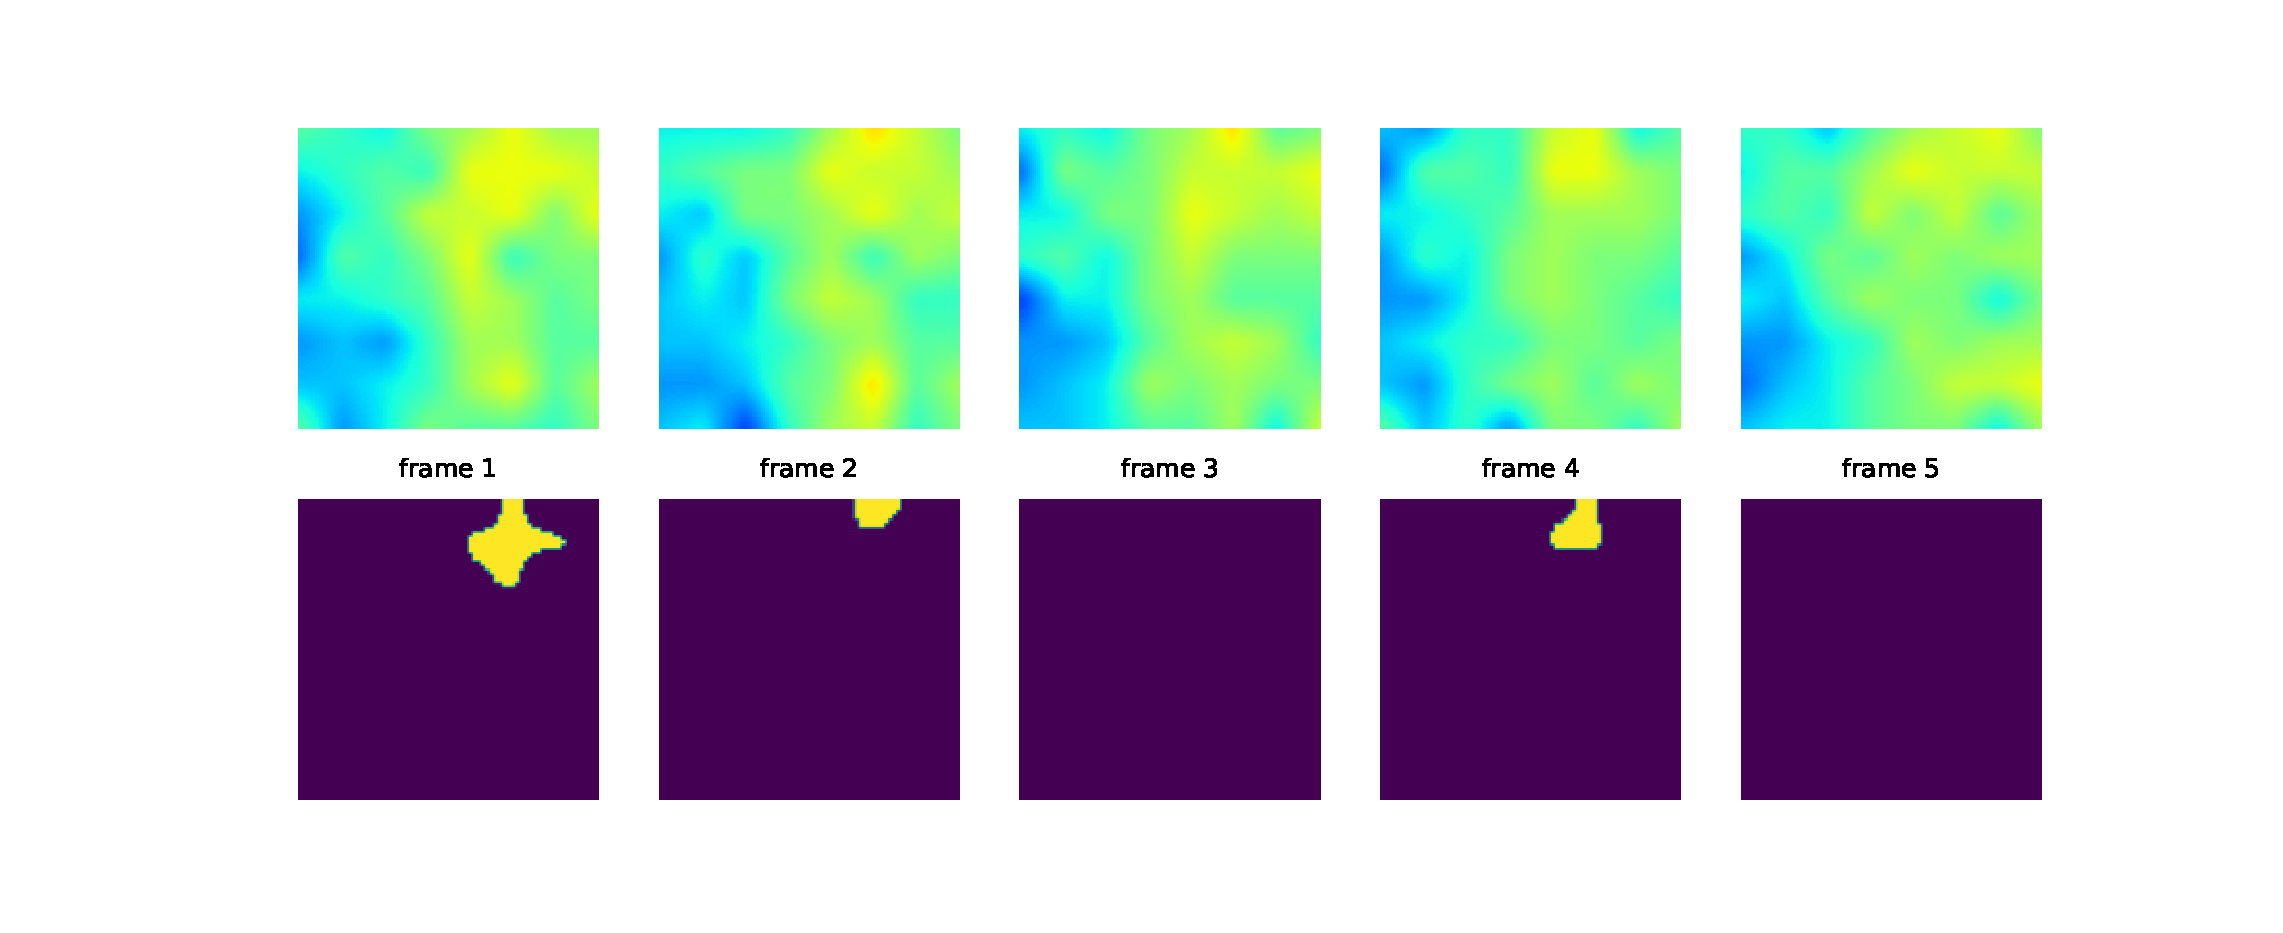
\includegraphics[width=\textwidth]{figures/err_noise1.eps}
  \caption{Sensor noises will not be tracked and counted even when they are incorrectly detected as objects because the sequence is usually not coherent.}\label{fig:err_no1}
\end{figure}
\begin{figure}
  \centering
  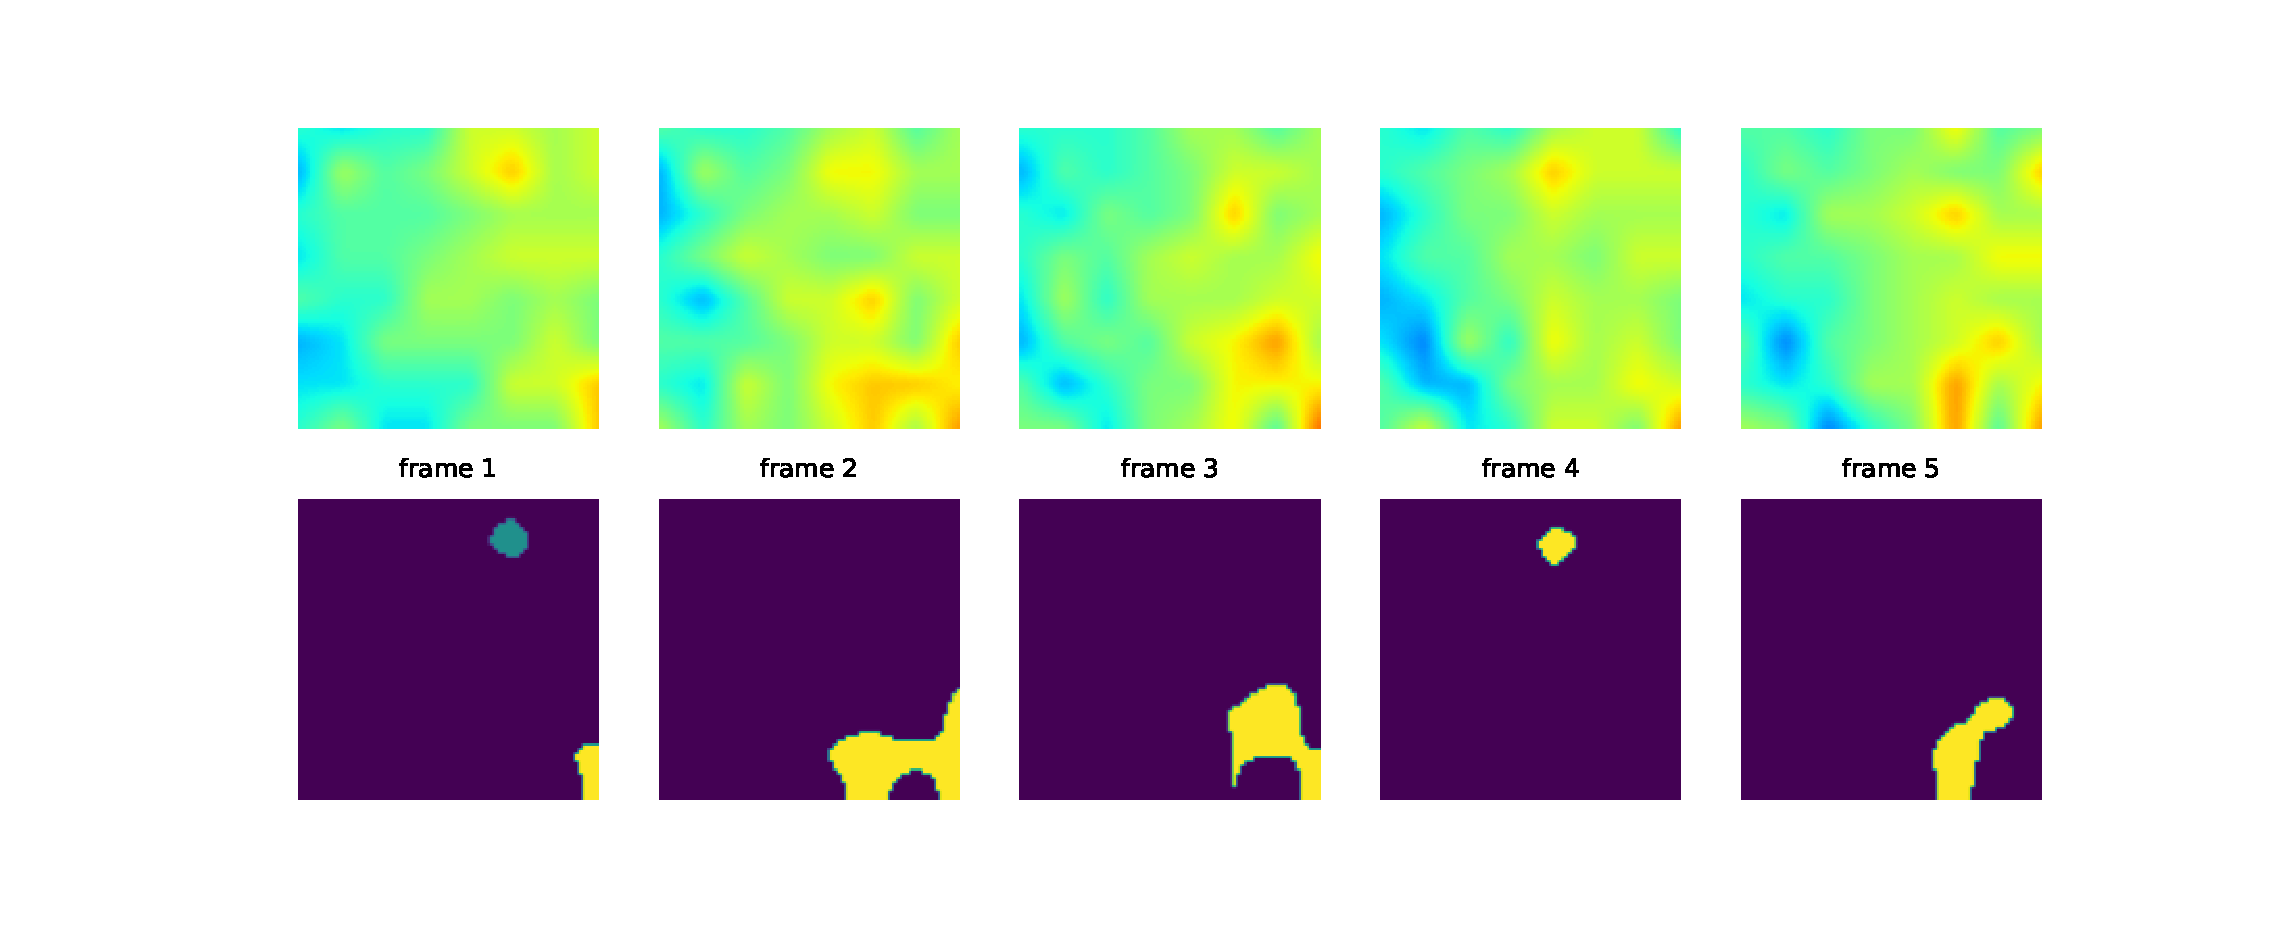
\includegraphics[width=\textwidth]{figures/err_noise2.eps}
  \caption{A noisy image sequence that may generate a wrong counting result. In the first 3 frames, the tracker has spawned an object in the right-bottom corner of the image. Later, the noise in frame 4 may be matched with the noise in frame 3, and the non-existing ``object'' has passed across the middle line. And in the next frame it disappears, which is considered as the termination of an exiting event. The human count is incorrectly decreased by one.}\label{fig:err_no2}
\end{figure}
Sometimes the temperature of a few pixels may temporarily exceed the segmentation threshold and be regarded as objects. The result is a few small objects emerging and disappearing randomly. We name this anomaly ``noise''. \autoref{fig:err_no1} shows an example of a noisy sequence. Fortunately, sensor noises usually will not cause a problem because they do not have an enter or exit tendency pattern as humans do. Tracking of a false detected noise pixel will fail within one or two frames and do not have an impact on the counting result. The only drawback is that the device will send too many rubbish messages to the storage platform if the camera is frequently activated by noises, which brings about the difficulty in debugging. Nevertheless, there are some noise sequences that cause a malfunction in the tracker, see \autoref{fig:err_no2}. When two noise trunks happen to emerge sequentially at different sides of the middle line, the tracking algorithm will take them as two frames of a moving object and generates incorrect results. Interestingly, we found that most of the problematic noisy sequences take place in the midnight when the ambient temperature drops. Therefore, the sensor noise issue should be traced back to the object detection layer. An improvement in \autoref{eq:detectionthreshold} may solve this problem.

Another potential issue takes place when a human stands under the camera for a long time, which is named as ``long sequence''. When there is an object in the camera view, the counting device needs to track it for every frame. The object must be segmented from the background over and over, the tracker needs to track the object even if it does not move at all, and the radio module keeps sending messages in minutes, which results in a lot of waste of computation power. Moreover, if a human occupies a certain area in the camera view, it increases the chance of incorrect matching when another person passes by. We have observed 6 long sequence anomalies during the real situation evaluation and all of them have been handled correctly.

Finally, the ``not detected'' issue describes when a human object passes under the camera but is not detected. This may happen when the human body temperature is too low, either because the body is covered by clothes or the person is short (the distance between camera and body enlarges for a short person, thus a lower detected body temperature). This issue can be solved by switching to a better IR camera with a larger detection range. It is also worth mentioning that the device only sends raw IR images for ground truth annotation when there are at least three pixels hotter than the room temperature. Therefore it is very likely that more events are not detected but also not noticed at all. This system bias in our experiment design can be solved by introducing another counting device based on different principles as a reference, for example, light barriers. An RGB camera may also help in collecting the ground truth if the privacy violation issue is lifted.

\section{Power Consumption}
The power consumption of the whole device is also an important aspect of the evaluation. The DHT11 temperature sensor consumes 1mA when measuring and 150µA when standby. The AMG8833 IR camera should run constantly and its average consumption is 4.5mA. \autoref{tab:esp32_power} shows the current consumption of the ESP32 in different modes. Without any power-saving tricks, the microcontroller consumes around 30mA (clock rate 160MHz) when idle and around 200mA when a human passes by. Assuming there are 40 enter and exit events every day and each event lasts 4 seconds (from image capturing until message publishing), the daily power consumption can be calculated approximately by \autoref{eq:power_estimate1}. On a common 600mAh Lipo battery, the device can operate for 16.5 hours, which is unsatisfying for an IoT application.
\begin{equation}\label{eq:power_estimate1}
\begin{split}
  P = (I_{esp32\ idle}+ I_{dht11}+I_{camera})mA * 24 hours + I_{esp32\ active}* t *n\\ \approx 852mAh +  9mAh = 860mAh
\end{split}
\end{equation}

It can be observed that though the radio module consumes the highest peak current, most of the battery power is wasted during the idle time because the device has to monitor the doorway all the time. To prolong the battery life, the key is how to reduce the power consumption when there is no event. Fortunately, Espressif provides many low-power options that can be integrated into our project. The light sleep mode can clock-gate the CPU and resume when an interrupt is triggered in the RTC peripheral. The deep sleep mode can power off the CPU totally to drastically reduce the power consumption lower than 1mA. Moreover, there is an 8MHz ultra-low-processor (ULP) along with the dual-core CPU that can retrieve sensor state and do some basic calculations when the main processors enter sleep mode, it can also wake up the main processors when necessary.

The power-saving design of our project contains two phases. The idle phase mainly contains the active pixel detection, i.e. the camera is polled by the ULP every 100ms to check if there is any pixel hotter than the environment temperature. And in the active phase, the ULP hands over the control of the camera to the main processors to track the object. To ensure an instant response of the human monitor device, we choose the light sleep mode because power up the main processors from deep sleep takes at least one second. Furthermore, we can neither afford the overhead of establishing the network connection whenever the main processor wakes up, so the RF module is kept powered on during sleep time. This results in power consumption of around 5mA during idle time. With the new idle current consumption, the daily consumption of the device is reduced to around 240mAh, and it can last around 2.5 days on a 600mAh battery.

More power is saved by deactivating the radio module so that the light sleep mode can be fully exploited. A constant network connection is required because the image data are too large to store in the internal memory, therefore we need to publish messages instantly. However, the image data are merely published for evaluation purpose and our algorithm works without the stored images. Without the image data, messages can be buffered in the memory and only send out once every hour. By this way we only bear the high current consumption during the relative short publish period and spare the expensive maintenance of the network. The estimated daily power consumption by this design is about 140mAh, see \autoref{eq:power_estimate2}. 
\begin{equation}\label{eq:power_estimate2}
\begin{split}
  P = (I_{esp32\ idle}+I_{camera})mA * 24 hours + I_{esp32\ active}* t_{event} *n \\+ I_{esp32\ publish}*t_{publish}*24\\ 
  \\\approx (1mA+ 4mA) * 24 hours + 40mA * (4s/3600) hours * 40 \\+ 180mA * 10s * 24
  \\= 120mAh +  8mAh + 12 = 140mAh
\end{split}
\end{equation}

By introducing additional sensors to detect approaching humans, the camera module no longer needs to operate constantly, which saves more power. For example, PIR sensors can be installed at both directions of the doorway to wake up the counting device in advance.   
The battery life can be further prolonged by deliberately shut down the device during midnight when it is unlikely to have any event.

\begin{table}[]
\centering
\begin{tabular}{|l|l|l|}
\hline
\textbf{Power mode}                  & \textbf{Description}            & \textbf{Power consumption} \\ \hline
Active (RF working)         & Wi-Fi transmit 802.11n & 180mA             \\
                            & Wi-Fi receive 802.11n  & 95 $\sim$100mA    \\ \hline
Active (RF not working)     & dual core 240MHz       & 30mA $\sim$68mA   \\
                            & dual core 160MHz       & 27mA $\sim$44mA   \\
                            & dual core 80MHz        & 20mA $\sim$31mA   \\ \hline
Light sleep with RF working & -                      & 5mA               \\
Light sleep                 & -                      & 0.8mA             \\ \hline
Deep sleep                  & ULP powered on         & 150µA             \\ \hline
\end{tabular}\caption{Power consumption of ESP32-WROVER module in different modes. The values are given by the ESP32 datasheet \cite{esp32datasheet} and confirmed by actual measurements.} \label{tab:esp32_power}
\end{table}

\section{Limitations}
The proposed algorithm has a few fundamental shortages. First of all, the object detection phase strongly depends on an accurate room temperature measurement and has a deterministic influence on the tracking result as the segmented object is the base of the following steps. Besides, the tracking algorithm based on central points can only handle multi-human events up to three or four people, if they were separated in the first few frames. The central point representation won't reflect the truth in crowded scenarios because multiple people will be regarded as one, for example, a large number of people crowding at the doorway when a meeting ends. Furthermore, our algorithm can not track a human who runs through the doorway, because the nearest neighbor matching method assumes the largest matching radius that is calculated from common walking speed.

There are also limitations to hardware. Currently, it takes around 20ms to process a single frame at a 160MHz CPU clock rate. The processing time may be longer if switching to a low-end MCU and eventually exceeds the time constraint. The program requires 953KB Flash and 220KB memory, the large memory requirement is mainly because of the image interpolation step. For images smaller than $71\times71$ resolution, the memory usage will likely remain the same. For larger images, both memory usage and process time will increase. 
\chapter{Conclusion and Future Works}
In this thesis, we have proposed a privacy-preserving human tracking algorithm, which receives top-view IR images as input and outputs the relative count of an enter or exit event at the doorway. The nature of low-resolution IR cameras prevents privacy violation fundamentally. We proposed to use a simple and effective segmentation threshold for object segmentation, use both centroids and central points to represent a binary blob, track the blob by nearest neighbor matching and finally filter the tracking result with an alpha-beta filter. The algorithm is capable to track single human passing through the doorway but also multiple humans at a common walking speed. We have deployed the algorithm on an ESP32-WROVER microcontroller and developed a doorway event counter that can operate independently for 2.5 days given the Wi-Fi infrastructure. The counted events are accumulated to obtain an estimation of building occupancy, which can be used in pandemic social distance regulation, HVAC optimization, and elder people caring.

Switching to a better IR camera that supports a longer detection range, higher resolution, and higher frame rate can enhance the algorithm accuracy as well as detect enter and exit events at various speeds. But the deployment cost will increase. Within the same hardware budget, a more complicated segmentation strategy has the largest potential to improve the counting result. The heat reflected from the surrounding environment poses a challenge in object segmentation and this should be taken into consideration in the development.
\backmatter
%\appendix{}
%\microtypesetup{protrusion=false}
% \glsaddall{} % add all defined terms to glossary, even if not referenced in text
% \printglossaries{} % TODO: uncomment if glossary needed
\listoffigures{}
\listoftables{}
\printbibliography{}

\end{document} 